\renewcommand{\appendixname}{Anexo}
\renewcommand{\thechapter}{\Alph{chapter}}

% Comando para iniciar la sección de anexos en el índice
\newcommand{\initappendix}{%
  \addcontentsline{toc}{chapter}{Anexo}%
}

% Comando para cada anexo individual
\newcommand{\anexo}[1]{%
  \refstepcounter{chapter}%
  \chapter*{Anexo \thechapter: #1}%
  \addcontentsline{toc}{section}{Anexo \thechapter: #1}%
  \markboth{Anexo \thechapter: #1}{}%
}

\initappendix

\anexo{Cronograma de Proyecto}

\section*{A.1 Diagrama de Gantt}
\addcontentsline{toc}{subsection}{A.1 Diagrama de Gantt}

El siguiente cronograma presenta la planificación pormenorizada del proyecto, organizada en cuatro fases principales con un total de veinte tareas distribuidas a lo largo del período marzo--diciembre de 2026. La granularidad adoptada es quincenal, identificando cada período como S1 (primera quincena) y S2 (segunda quincena) dentro de cada mes. Para cada tarea se especifica su tarea predecesora en la columna ``Dep.'', lo que permite visualizar las dependencias técnicas entre actividades y evaluar el impacto de eventuales desvíos sobre la ruta crítica del proyecto.

\begin{figure}[ht]
    \centering
    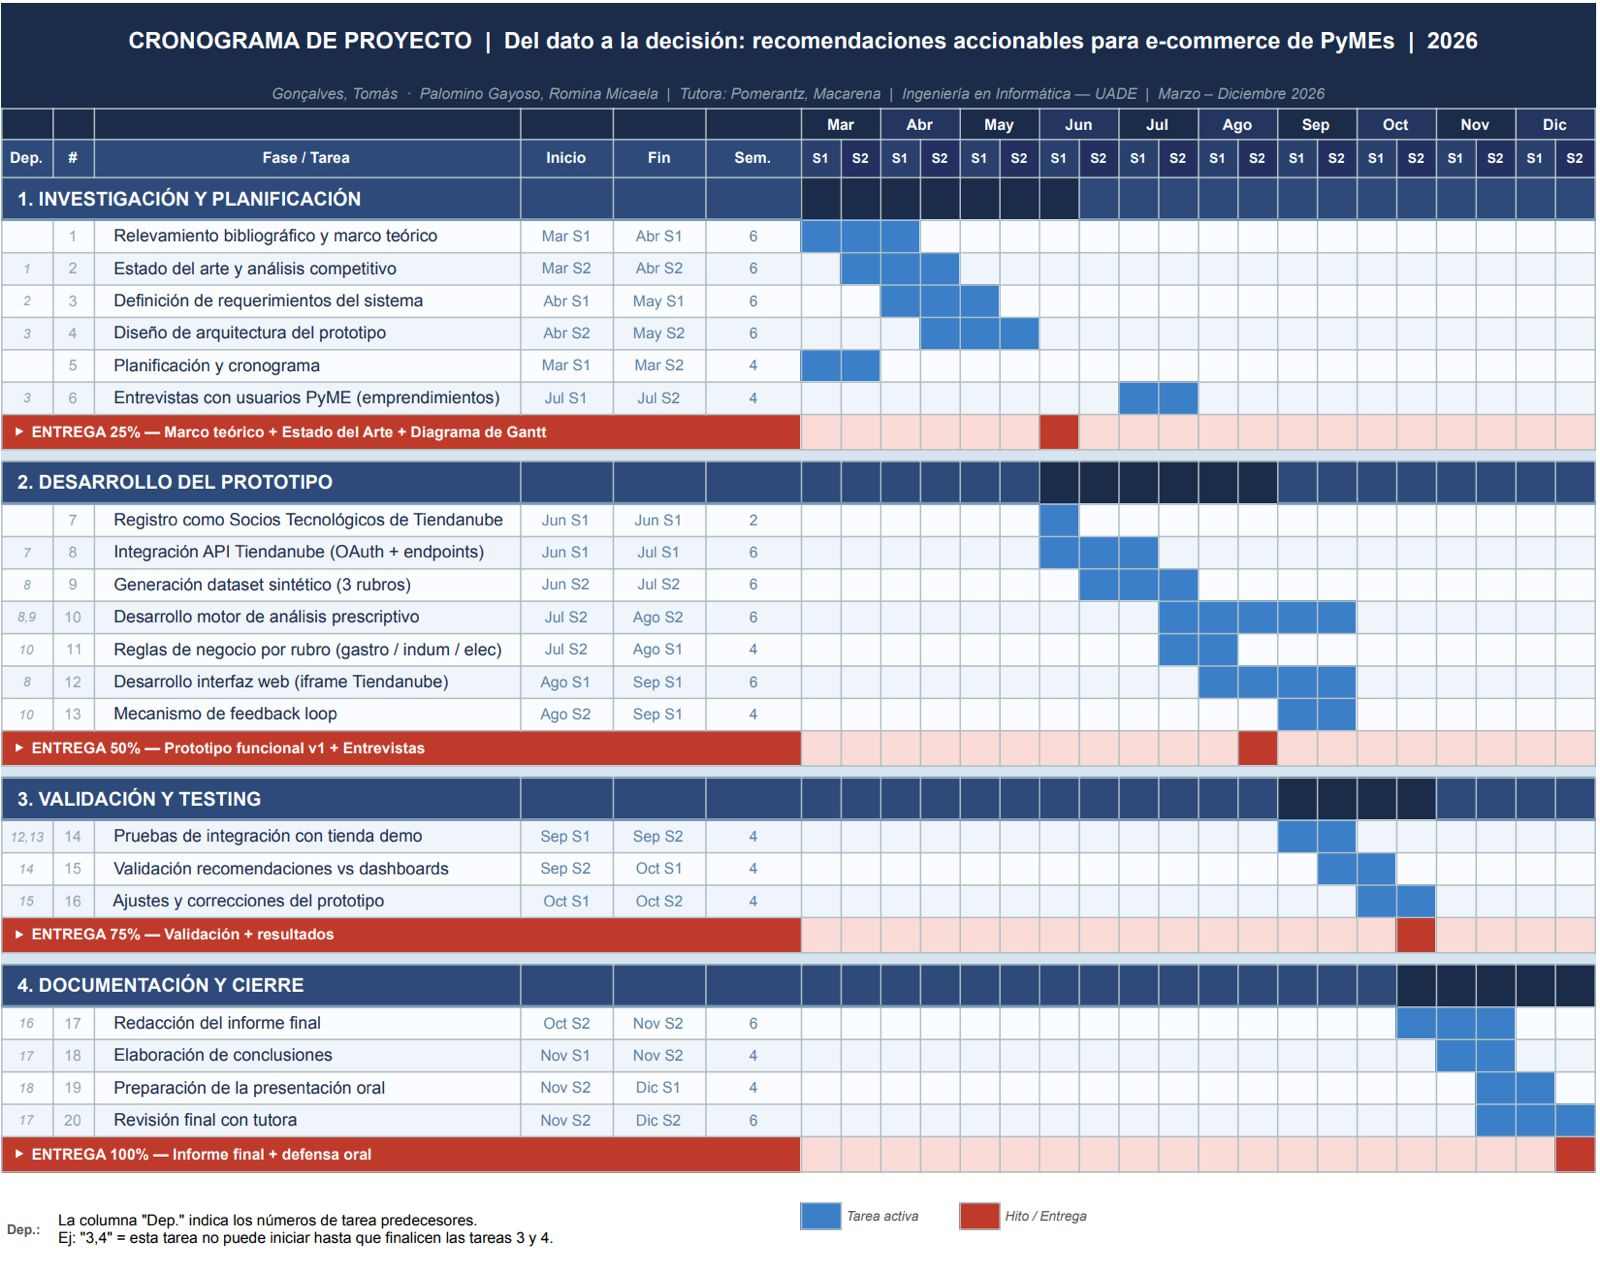
\includegraphics[width=\textwidth]{./gantt/gantt_pfi_palominoGoncalves.jpeg}
    \caption{Cronograma de proyecto --- Diagrama de Gantt.}
\end{figure}

\noindent\textit{Fuente: elaboración propia. El archivo editable con detalle quincenal completo se encuentra disponible en \href{https://docs.google.com/spreadsheets/d/1RAgiah4WoOmxSgkorFZD4-IMevJZzECZ6DJtNFgUqrY/edit?usp=sharing}{este enlace (Google Sheets)}.}

\section*{A.2 Justificación técnica de desvíos anticipados}
\addcontentsline{toc}{subsection}{A.2 Justificación técnica de desvíos anticipados}

Al momento de la presente entrega (25\%), el proyecto se encuentra dentro de los plazos planificados. No obstante, se identifican a continuación los principales riesgos de desvío temporal, junto con las estrategias de mitigación previstas para cada uno.

\bigskip
\noindent\textbf{Desvío potencial 1 --- Registro como Socia Tecnológica de Tiendanube (Tarea 7)}

El proceso de registro en el programa de Socios Tecnológicos de Tiendanube es un prerrequisito directo para las tareas de integración con la API (Tarea 8) y, en cascada, para el desarrollo del motor de análisis (Tarea 10) y la interfaz web (Tarea 12). En caso de que los tiempos de aprobación por parte de Tiendanube superen los estimados, se adelantará el desarrollo del dataset sintético (Tarea 9), que puede ejecutarse de forma independiente, evitando así el bloqueo de la ruta crítica del desarrollo.

\bigskip
\noindent\textbf{Desvío potencial 2 --- Entrevistas con usuarios PyME (Tarea 6)}

La concreción de entrevistas con propietarios de emprendimientos y comercios de pequeño y mediano tamaño depende de la disponibilidad de terceros, lo que introduce incertidumbre en su planificación. Por esta razón, las entrevistas se planificaron para la primera quincena de julio, con margen suficiente para ser incorporadas en la entrega del 50\% en caso de no completarse en la fecha prevista.

\anexo{Transcripciones de entrevistas}

\subsection*{B.1 Entrevista N.°~1 --- Delfina Fernández}
\addcontentsline{toc}{subsection}{B.1 Entrevista N.° 1 --- Delfina Fernández}

\noindent\textbf{Entrevistada:} Delfina Fernández\\
\noindent\textbf{Perfil:} Dueña de emprendimiento de indumentaria bordada a mano (remeras y musculosas). Vende por Instagram y Tienda Nube. También trabaja en armado de pedidos de tienda online (otra empresa).\\
\noindent\textbf{Entrevistadores:} Tomás Gonçalves (moderador) y Micaela Palomino (observadora)\\
\noindent\textbf{Fecha:} Domingo 31 de mayo de 2026\\
\noindent\textbf{Modalidad:} Videollamada (semiestructurada)\\
\noindent\textbf{Plataforma del negocio:} Tienda Nube (primer nivel pago)

\begin{framed}
\small\noindent\textit{Nota metodológica: Esta transcripción fue limpiada a partir de la grabación original. Se eliminó charla trivial previa y posterior a la entrevista, se corrigió la sintaxis para mejorar la fluidez de lectura y se reasignaron las atribuciones de orador en casos donde la herramienta de transcripción automática las asignó erróneamente (verificado por contexto). No se agregó, inventó ni dedujo información que los participantes no hayan dicho explícitamente. La entrevistada cuenta con un colaborador (Facundo) que interviene brevemente mostrando una aplicación personalizada.}
\end{framed}

\subsubsection*{Bloque 0 · Introducción y rapport}

\noindent\textbf{Micaela Palomino:} Nuestro proyecto, nuestra tesis, trata de hacer un agente y conectarlo a Tienda Nube. Me acordé de que vos tenés un emprendimiento en Tienda Nube, así que nos viniste a escuchar.

\noindent\textbf{Delfina Fernández:} Sí, yo te iba a decir, tengo un poco de miedo porque en realidad no sé qué tanto uso Tienda Nube. Pero igual trabajo con Tienda Nube; mi trabajo es con Tienda Nube. Así que bueno.

\noindent\textbf{Micaela Palomino:} La entrevista la va a llevar Tommy, así que todo tuyo, Tommy.

\noindent\textbf{Tomás Gonçalves:} Arranquemos de base, porque yo no conozco. Delfina, ¿de qué es tu negocio? ¿Qué vendés?

\noindent\textbf{Delfina Fernández:} Yo tengo un emprendimiento ---en realidad, porque es chiquito todavía--- en el que hago remeras y musculosas bordadas a mano. Por ahora es eso. Tengo mi página de Instagram y también mi página de Tienda Nube para vender por ahí. La verdad es que vendo por los dos lugares, pero Tienda Nube sirve mucho.

\subsubsection*{Bloque 1 · Contexto del negocio y herramientas actuales}

\noindent\textbf{Tomás Gonçalves:} Me acuerdo que dijiste que empezaste en Tienda Nube, pero como que no sabés usarlo tanto en la parte de datos.

\noindent\textbf{Delfina Fernández:} A ver, no es que tengo un máster en Tienda Nube. Con el emprendimiento no lo uso tanto. Las ventas, quizás por ahora, las estoy haciendo más en el boca a boca. Pero en mi trabajo, trabajo con todo lo que es armado de pedidos de tienda online. Entonces, ahí sí uso Tienda Nube, todo el tema de stock y demás.

\noindent\textbf{Tomás Gonçalves:} De la data que te ofrece Tienda Nube, ¿le das mucha pelota?

\noindent\textbf{Delfina Fernández:} Me imagino que tiene que tener estadísticas, tema de ventas. Eso por ahora no tanto, porque recién ahora empecé a pagar el primer nivel, que es el que te da más datos, más opciones para métodos de pago y métodos de envío. Todavía no lo uso tanto, pero porque tampoco lo tengo linkeado con Instagram, que creo que se puede hacer. Así que veo, por ejemplo, cuántas visitas tuve en el día, y esas cosas.

\noindent\textbf{Micaela Palomino:} Vos entrás en la Tienda Nube del emprendimiento. Básicamente lo que hacés es cargar el stock que tenés. ¿Y después cómo es todo el flujo? ¿Te llegan las ventas? ¿Se gestionan por Tienda Nube? ¿Vos tenés que entrar a ver qué ventas se realizaron, o te llega un mail?

\noindent\textbf{Delfina Fernández:} Me llegan las dos cosas. Cuando llega una venta me llegan tres notificaciones más un mail o dos, si el pago ya está recibido. Yo el stock ahí no lo tengo cargado todo, porque como son productos que tardo bastante en hacer, me da miedo cargar cinco remeras de un modelo y que me compren las cinco en la misma semana cuando ya tengo diez ventas y no las puedo entregar a tiempo. Entonces eso lo voy gestionando yo: pongo uno o dos de cada uno, y cuando veo que alguien me compra y ya no tengo stock de eso, lo doy de baja. Yo me manejo con las musculosas: quizás tengo la blanca en distintos modelos, pero en realidad tengo cinco modelos de bordado y dos remeras blancas nada más. Entonces, cuando me compran una, ya tengo que estar atenta a la próxima compra para darla de baja, porque no tengo otra.

\noindent\textbf{Micaela Palomino:} Y cuando te hacen una compra, ¿vos tenés que entrar a Tienda Nube a fijarte que te quedaste sin esto y volver a recargarlo? ¿Es todo manual, o te dice que te quedaste sin stock?

\noindent\textbf{Delfina Fernández:} Me lo dice. Las tres notificaciones que me llegan son: tenés una nueva compra (que más o menos te dice qué te compraron y quién), después me llega otra que dice que me quedé sin stock de ese producto exacto, y si ya pagaron, el pago recibido. Además me llega mail de la compra y mail del pago recibido.

\noindent\textbf{Micaela Palomino:} ¿Y te avisa antes de quedarte sin stock? Cuando te queda una prenda, ¿no te avisa?

\noindent\textbf{Delfina Fernández:} No, no, no. Eso no.

\noindent\textbf{Tomás Gonçalves:} O sea, es todo dinámico: te llega la alerta de que te quedaste sin stock y decís, bueno, me toca reponer.

\noindent\textbf{Delfina Fernández:} Claro, literalmente.

\noindent\textbf{Tomás Gonçalves:} ¿Y entre que te quedaste sin stock y reponés, cuánto tiempo pasa?

\noindent\textbf{Delfina Fernández:} Depende de cuándo hagan la compra. Si lo hacen durante el día, lo hago rápido: me fijo si sigo teniendo stock de eso y agrego otra más. Pero, por ejemplo, el otro día me desperté y había una compra de muy temprano; era sábado, como a las ocho de la mañana. Yo hasta las once no abrí los ojos, la vi, y ahí recién repuse el stock. Pero si no, es rápido.

\noindent\textit{--- Métricas y estadísticas de Tienda Nube ---}

\noindent\textbf{Micaela Palomino:} Me quedé con lo que decías de las visitas, que era una métrica que te da Tienda Nube. ¿Cómo es? ¿Te llega por mail o solamente por Tienda Nube?

\noindent\textbf{Delfina Fernández:} Es la parte de inicio en Tienda Nube. Hay como un cuadrito con cuatro cosas, y podés poner el período: ver ese cuadro basado en hoy, ayer o la semana entera. Ahí es donde dice visitas únicas en el día. Yo siempre lo tengo puesto por el día, pero se puede ver por otros períodos también.

\noindent\textbf{Micaela Palomino:} ¿Y esto te sirve para algo? ¿Después podés llevar esto a una acción?

\noindent\textbf{Delfina Fernández:} Yo creo que sí. Todavía no sé si lo apliqué, pero por ejemplo, me pasó de subir un posteo con un modelo nuevo de bordado, y ese día tuve como diecisiete vistas, que fue un montón. Y después nunca más volví a ver tantas. En cambio, el otro día volví a subir un posteo con las del Mundial, y ahí otra vez subió bastante. Entonces dije: quizás le tengo que meter mucho más a los posteos, y las historias también generan bastante tráfico. Voy tanteando.

\noindent\textbf{Micaela Palomino:} ¿Y después hubo conversión más allá de las visitas? ¿Tuviste más visitas y aumentaron las ventas, o no necesariamente?

\noindent\textbf{Delfina Fernández:} Eso lo estaba pensando el otro día. No sé si va muy de la mano, porque por ejemplo, ese día que tuve diecisiete visitas quizás no tuve venta o tuve una sola. Y el otro día, con el posteo del Mundial, tuve nueve visitas y tuve dos o tres ventas en un día. No sé cómo va eso de la mano.

\noindent\textbf{Tomás Gonçalves:} La cantidad de ventas está atada a lo que haya en el momento, más o menos. Con el Mundial te vino re bien, entonces.

\noindent\textbf{Delfina Fernández:} Sí, re contra. Pero es que el modelo anterior tuve diecisiete visitas y no me compró nadie. En cambio, con este tuve nueve visitas, que fue mucho menos, y tuve tres ventas.

\noindent\textbf{Micaela Palomino:} ¿Qué otras métricas te muestra Tienda Nube además de visitas únicas?

\noindent\textbf{Delfina Fernández:} A ver, me fijo. Te muestra visitas únicas, ventas, facturación y ticket promedio. Se puede filtrar por hoy, ayer y esta semana.

\noindent\textit{[Delfina comparte pantalla mostrando el panel de inicio de Tienda Nube]}

\noindent\textbf{Delfina Fernández:} Este es el inicio. Lo del principio es para mí, lo que tengo que ir marcando: sin ventas por cobrar (porque hay veces que te pagan otro día; Tienda Nube te da hasta tres días para poder pagar por transferencia, y si no, te cancela la compra), cuatro ventas por empaquetar (que son todavía las que no hice), lo mismo con enviar y por retirar. Eso es para ordenarme. Y después están las métricas que les iba diciendo: visitas únicas, ventas, esta semana, ayer. Ustedes díganme qué quieren que aprete, porque yo no tengo idea.

\noindent\textit{--- Seguimiento de ventas y herramientas complementarias ---}

\noindent\textbf{Micaela Palomino:} ¿Vos le das seguimiento a las ventas o solamente lo tenés concentrado acá en Tienda Nube? Por ejemplo, ¿sabés cuál es la remera que más vendiste, o cuál es el diseño que más vendés?

\noindent\textbf{Delfina Fernández:} En Tienda Nube yo sé que si pagás los niveles más pro ---esto lo sé por mi trabajo---, podés ver todo eso. Yo no lo tengo acá porque pago el nivel uno. Igual, yo hago el seguimiento. Antes lo hacía por Tienda Nube: me iba anotando todo. Es más, las ventas que me hacían por boca a boca yo igual las simulaba en Tienda Nube. Pero ahora Facundo me hizo una app, entonces guardo todo ahí; voy marcando todo ahí.

\noindent\textbf{Micaela Palomino:} ¿Y la app que te hizo Facundo, qué seguimiento le das? ¿Para qué métricas la usás?

\noindent\textbf{Delfina Fernández:} Las ventas las cargo todas ahí. Después también me hizo como parte del proceso de producción: yo voy marcando si ya está bordada, si se va a lavar, después a planchar, después a empaquetar y después ya está entregada. Y todo el tema de los ingresos y egresos también los marco ahí. Todas las remeras que compro, las veces que compro, las marco ahí, y después se va haciendo toda la cuenta sola.

\noindent\textit{[Facundo, colaborador de Delfina, muestra brevemente la sección de analytics de la app]}

\noindent\textbf{Facundo (colaborador):} En Analytics tenemos todo lo de los ingresos totales, egresos totales, balance neto por mes y por semana. Después también está la parte de ver cuál es la que más se vende.

\subsubsection*{Bloque 2 · Gestión de inventario y stock}

\noindent\textit{--- Publicidad y temor al quiebre de stock ---}

\noindent\textbf{Tomás Gonçalves:} ¿Hacés publicidad?

\noindent\textbf{Delfina Fernández:} Todavía no. Ese es mi próximo paso. Literalmente esta semana estoy tratando de organizarme para ver qué necesito hacer primero. El tema es que yo tardo en hacer cada producto. Ahora, ponele, ya sé cuál es mi límite de ventas que puedo tener por semana: son las remeras que yo llego a hacer. Si no, las entrego tarde. Ahora estoy en el límite, por suerte. Entonces, si pongo publicidad, un poco de miedo me da de que se vaya todo a la mierda.

\noindent\textbf{Tomás Gonçalves:} Alto miedo. ¿Cómo es el tema de las publicidades? Me imagino que tenés que estar bien preparada.

\noindent\textbf{Delfina Fernández:} Claro, porque en el otro lugar donde trabajo, antes pasaba eso: era activar publicidad y a los dos días darla de baja porque decíamos que ya no dábamos abasto. Entonces un poco de miedo tengo.

\noindent\textbf{Tomás Gonçalves:} Es como que tenés que estar pendiente del stock y todo eso.

\noindent\textbf{Delfina Fernández:} Sí, eso es lo que me mata, porque todavía no tengo un stock tremendo. Entonces me tengo que estar muy encima.

\noindent\textit{--- Quiebre de stock y reposición de insumos ---}

\noindent\textbf{Micaela Palomino:} ¿Con los modelos de bordado te pasa lo mismo de guiarte por intuición?

\noindent\textbf{Delfina Fernández:} Los modelos de bordado no; eso sí me doy cuenta más por lo que pidieron. Por ejemplo, yo sé que el pimiento y las aceitunitas se venden mucho. Llegó un momento en que me estaba quedando sin mostacillas rojas para el pimiento y dije: ¿qué hago ahora? No las conseguía, no las conseguía. Me compré una bolsa grande, y ahora nadie me pide más el pimiento porque vino el invierno. Pero sí, eso también lo veo por la app de Facundo, que ahí tengo el orden de las que más fui vendiendo. Por ejemplo, ahora me estoy quedando sin mostacillas de otro color que no vendo tanto, y digo: bueno, ya está.

\noindent\textbf{Micaela Palomino:} Si hubieses sabido que la de pimiento se iba a vender más, ¿hubieses comprado de antemano más mostacillas? ¿Te pasó alguna vez que vendiste más de lo que pensabas?

\noindent\textbf{Delfina Fernández:} Sí, me pasó justamente con el pimiento y con las aceitunitas. Me quedé sin mostacillas y dije: tengo que salir ya a comprar, porque no tenía, y no pensé que se iban a vender tanto. De la nada, en una o dos semanas, las aceitunitas era la única que me pedían.

\noindent\textbf{Tomás Gonçalves:} Claro, te enterás en el momento cuando ya se agotó.

\noindent\textbf{Delfina Fernández:} Claro, yo voy tanteando cuánto tengo, pero es como que nunca se sabe qué venta va a entrar.

\noindent\textbf{Tomás Gonçalves:} Entonces, proyectar cuántas ventas vas a tener la semana que viene es imposible.

\noindent\textbf{Delfina Fernández:} Con los modelos anteriores, que tenía varios y eran todos de verano, sí, era más difícil. Ahora que estoy con las del Mundial, hice tres modelos. Hay uno que me lo pidieron una sola vez; los otros dos están muy peleados. Igual, sé que me pedían mucho más la de Argentina que la de las Carapela, por ejemplo. Pero no te puedo decir con métricas; es más intuición. También me doy cuenta cuando subo historias o posteos a Instagram y me contestan bastante: me contestan más una que la otra, y voy por ahí.

\subsubsection*{Bloque 3 · Análisis de ventas y decisiones comerciales}

\noindent\textit{--- Patrones de venta y estacionalidad ---}

\noindent\textbf{Micaela Palomino:} ¿Sabés qué día es el que más vendés?

\noindent\textbf{Delfina Fernández:} No, eso por ahora está como muy difuso. Yo creo que ni la app lo podría captar, porque es muy variable. Por ejemplo, vendo más del boca en boca: voy a Pilates y llevo una para que alguien se pruebe, y ya ahí vendo tres. Entonces quizás te puedo decir que los jueves que voy a Pilates vendo, pero de repente un jueves subo un posteo y la gente me compra tres en un día también por Tienda Nube. Por ahora no sé si hay tantas ventas como para decir que un día es el que más compran. Sí puedo decir horarios: me compran más a la mañana, entre las ocho y las once, o a la noche, tipo ocho o nueve. Es como que la gente o termina el día y se pone a comprar, o se levanta y se pone a comprar.

\noindent\textbf{Tomás Gonçalves:} Con el Mundial, ¿vos dijiste ``voy a lanzar un producto relacionado a eso'', o sacás productos random?

\noindent\textbf{Delfina Fernández:} Los modelos nuevos los venía sacando random: si encontraba alguno que me gustaba y me emocionaba hacerlo, lo hacía y lo sacaba. Pero con las del Mundial dije: sí, algo tengo que hacer, porque se va a vender. Este año igual hay cero emoción de Mundial, como se habrán dado cuenta, pero vienen bien. Tengo tres modelos, varían los tipos de remera también, y se viene vendiendo bien. Fue tipo una cápsula mundialista.

\noindent\textit{--- Política de precios ---}

\noindent\textbf{Micaela Palomino:} ¿Cómo van los precios? ¿Te basás en algo? ¿Los ajustás?

\noindent\textbf{Delfina Fernández:} Eso es un tema que me cuesta mucho. Para arrancar, en noviembre, sacamos los costos (lo hizo Facundo). Yo no quería que fuera una prenda cara, porque sé que siendo un Instagram de trescientos seguidores, y aparte al principio siempre te compran los conocidos, me cuesta ponerle un precio alto. Los precios los mantengo lo más que puedo por ahora; los puse desde el principio y no se movieron mucho. Cuando fui sumando otro tipo de remeras que están más caras, ahí sí o sí esa diferencia se la sumo, porque si no me la como yo. No es lo mismo una musculosa que una remera boxy fit.

\noindent\textit{--- Datos concretos versus intuición ---}

\noindent\textbf{Micaela Palomino:} Hoy en día, ¿cuántas de las decisiones que tomás para el emprendimiento están basadas en datos concretos y cuántas en la intuición y experiencia? Por ejemplo, cuando tenés que hacer una compra de remeras, ¿comprás porque tenés datos de que se van a vender, o más por intuición?

\noindent\textbf{Delfina Fernández:} Un poco y un poco. Por ejemplo, ya sé que el talle M es el que más me piden, entonces ahí sí sé por qué: es el que más pidieron. Y a la vez, si alguien quería un S, le ofrezco el M porque sé que no es una gran diferencia, y lo mismo con el L. Después, el negro no se vendió tanto como la blanca, porque también tengo muchos más modelos de bordado que van más con la blanca que con la negra. Pero sí, es un poco y un poco por ahora.

\subsubsection*{Bloque 4 · Puntos de dolor y visibilidad del negocio}

\noindent\textbf{Tomás Gonçalves:} A mí me asustaría la incertidumbre: no saber qué vendo, qué no vendo.

\noindent\textbf{Delfina Fernández:} Sí, también te cuento: hice una promoción con las del Mundial. Dije que si me compran esta remera y ganamos la cuarta, les guardo la cuarta estrella gratis. Pero solo una persona me la compró. Tampoco sé si me conviene, porque es la que más tardo en hacer. Así que lo voy a pensar.

\subsubsection*{Bloque 5 · Validación de la propuesta de valor}

\noindent\textit{--- Recomendaciones de reposición ---}

\noindent\textbf{Tomás Gonçalves:} Imaginá que Tienda Nube te ofrece una opción que, en base a tu historial, te dice: ``Te conviene reponer X producto antes del fin de semana porque el sábado vas a tener unas ventas esperadas de veinte unidades.'' ¿Te coparía tener algo así?

\noindent\textbf{Delfina Fernández:} Eso estaría buenísimo, porque más que nada a mí me sirve por el material. Nunca sé si comprar más o si me los voy a quedar sin vender. Entonces me sirve por eso, porque si termino comprando algo que no lo voy a vender, es pérdida. Eso sería buenísimo.

\noindent\textit{--- Visibilidad por producto ---}

\noindent\textbf{Micaela Palomino:} Vos lo que decías era que te guiabas por la intuición, pero en realidad la intuición es la interacción que tenés en Instagram. Después nos contabas que en Tienda Nube te aparecen las visitas únicas, pero no te dice específicamente de qué producto. Si te dijera que hoy hiciste un posteo y tuviste quince visualizaciones, y las quince fueron de determinado producto, tal vez es un índice de que ese producto probablemente lo vendas.

\noindent\textbf{Delfina Fernández:} Sí, eso estaría buenísimo también. Estaría muy bueno.

\noindent\textbf{Delfina Fernández:} Ahora estoy con el primer nivel pago de Tienda Nube. Estaba con el que es gratis y no te daba nada de métricas. Recién el mes pasado lo empecé a pagar.

\noindent\textit{--- Descripción de la propuesta y reacciones ---}

\noindent\textbf{Tomás Gonçalves:} La herramienta que más o menos te describimos, ¿qué valor le darías? ¿Cuánto pagarías por algo así?

\noindent\textbf{Delfina Fernández:} ¿Solo por eso, o si viene incluido en Tienda Nube?

\noindent\textbf{Micaela Palomino:} Lo que pensábamos era armar un agente que se conecte a Tienda Nube, pero que ofrezca acciones concretas. No eso de ``tuviste cinco visitas'' y vos decís: ¿qué hago ahora? Sino más bien: aumentá el stock de esto, dejá de comprar mostacillas de las tres estrellas porque nadie entró a verlas, los días jueves son los que más vendés (o al revés: los miércoles son los que menos vendés, entonces poné un descuento para que los miércoles la gente entre). Datos más concretos, acciones en vez de métricas. Decirte exactamente lo que tenés que hacer para aumentar lo que vos quieras, dependiendo de tu objetivo: puede ser aumentar las ventas, o quizás sos más conservadora y preferís vender todo el stock. Pensamos dos formas: una era que se conecte directamente a Tienda Nube, porque entendemos que la gente quizás no quiere usar dos herramientas.

\noindent\textbf{Delfina Fernández:} No, y aparte es que los clientes entran a la página online, que es Tienda Nube. Entonces está bueno que agarre toda la información de ahí, porque ahí es donde se vende.

\noindent\textbf{Micaela Palomino:} La otra opción era armar una plataforma separada que haga lo mismo. Lo estamos pensando.

\noindent\textbf{Delfina Fernández:} Está buenísimo. Con todos estos datos hay infinidad de cosas que podés hacer: desde poner descuentos, meter publicidad solo con esa remera, subir un millón de posteos ese día. Está buenísimo. Y aparte, sirve, porque yo quizás veo las diecisiete vistas y digo: ay, qué bueno, se re pegó este posteo. Después hubo otro igual o parecido y no se pega, y no tengo esas vistas. Entonces digo: ¿qué hago?

\noindent\textbf{Micaela Palomino:} Siempre es el mismo problema: no entendés por qué fueron esas quince vistas. Si te dijéramos que fueron por tal cosa, ya sabés qué patrón repetir o qué posteo funciona.

\noindent\textbf{Delfina Fernández:} Sí, y también de dónde vienen las visitas. Quizás vienen del perfil, o quizás vienen de la historia que subí. Eso está buenísimo.

\noindent\textbf{Micaela Palomino:} Por ejemplo, si alguien comparte tu link por WhatsApp, no es lo mismo que entre por un posteo tuyo. Sabés que funciona el boca en boca, y después sabés que tenés más conversión por los posteos, entonces decís: le tengo que dedicar un poquito más a los posteos.

\noindent\textit{--- Disposición a pagar ---}

\noindent\textbf{Delfina Fernández:} Bueno, contestando a la pregunta de cuánto pagaría: yo ahora estoy pagando veintisiete mil pesos. Yo creo que entre cuarenta y cincuenta mil pagaría si viene con esto, porque es lo que me va a terminar de dar la devolución de lo que estás haciendo; es lo que me estaría faltando ahora. Así que sí, yo creo que lo vale. No me acuerdo cuánto está el próximo plan de Tienda Nube; no sé si estaba como setenta u ochenta mil. No sé qué tiene tampoco, no me puse a fijar. Pero creo que es un muy buen extra.

\subsubsection*{Bloque 6 · Cierre}

\noindent\textbf{Micaela Palomino:} Más allá de todo lo que te contamos que queremos hacer, si te damos la posibilidad de decirnos qué te gustaría que hagamos: ¿qué otras funcionalidades te gustaría que tenga?

\noindent\textbf{Delfina Fernández:} Es muy difícil para contestar ahora.

\noindent\textbf{Micaela Palomino:} ¿Qué es lo que más te cuesta hoy, que decís: por favor, resuélvanme esto?

\noindent\textbf{Delfina Fernández:} Quizás el tema publicidad. Todo lo que me venís nombrando es literalmente lo que me venía haciendo ruido, porque no sé cuándo, es todo incertidumbre: no sé cuánto voy a vender, cómo, qué. Quizás que me ayude con el tema publicidad: ``tengo floja esta remera'', que me lo avise y yo le pongo toda la publicidad del mundo a esa remera. O que me prediga cuánto voy a vender de tal modelo esta semana, que puede ser como el boom; así subo la publicidad al máximo o la bajo. Eso está buenísimo. Ahora no se me ocurre algo extra, porque siento que de verdad está muy bueno lo que me estaban contando. No sé si le falta algo por ahora.

\noindent\textbf{Micaela Palomino:} Siento que sería muy bueno que, en vez de recibir el pedido para ponerte a hacer el diseño y el bordado, lo podrías hacer de antemano y ya los tendrías preparados para cuando te lo pidan.

\noindent\textbf{Delfina Fernández:} Sí, eso sería buenísimo. Aparte hay baches de ventas. Antes del Mundial estaba medio sin saber qué hacer y me puse a hacer un par de antemano. Ahora me resolvió la vida, porque de la nada en una semana vendí diez o doce, y digo: las tengo que hacer todas para la semana que viene, pero ya tenía un par hechas. Eso resuelve de muchas maneras.

\noindent\textbf{Tomás Gonçalves:} Por ahora está muy completo. Pero capaz que nosotros nos salteamos algo. ¿Hay algo que quieras saber o que te gustaría que hayamos preguntado?

\noindent\textbf{Delfina Fernández:} No tenía expectativas; es más, tenía un poco de miedo. Si me preguntan mucho de métricas y esas cosas que yo todavía no me acostumbro a usar, porque ni siquiera pago publicidad, dije: ay, ¿qué voy a hacer? Pero creo que estuvo bastante bien. Me gustó mucho lo que me están contando de qué van a hacer. El concepto ya me encantó: esto de que se va a acabar la incertidumbre, que es lo que te mata un poco.

\noindent\textbf{Delfina Fernández:} Se me ocurre también poder linkearlo con Instagram. Quizás como poder ver: este posteo está hecho de tal y tal manera, y esto es lo que funcionó. Sacar datos de ahí también, para decir: esto vendió.

\noindent\textbf{Delfina Fernández:} Yo ahora me estoy manejando mucho más con Instagram que con Tienda Nube, porque no termino de usar Tienda Nube bien. Dice cosas y digo: ¿qué hago con esto? En Instagram es todo un tema. Todavía no pago publicidad, y estaría bueno que si pago esto de Tienda Nube, tenerlo linkeado con Instagram y ver qué sale de ahí.

\noindent\textbf{Micaela Palomino:} Muchas gracias por el aporte y por conectarte un domingo a la noche.

\noindent\textbf{Delfina Fernández:} Cualquier cosa me dicen, yo no tengo problema.

\noindent\textbf{Tomás Gonçalves:} Muchas gracias por todo.

\begin{center}\textit{--- Fin de la entrevista ---}\end{center}

\subsection*{B.2 Entrevista N.°~2 --- Morena Cejas}
\addcontentsline{toc}{subsection}{B.2 Entrevista N.° 2 --- Morena Cejas}

\noindent\textbf{Entrevistada:} Morena Cejas\\
\noindent\textbf{Perfil:} Dueña de emprendimiento de indumentaria (ropa unisex: remeras, bermudas, buzos, joggings). Vende por Instagram, boca en boca y Tienda Nube. Tiene menos de un año de antigüedad.\\
\noindent\textbf{Entrevistadores:} Tomás Gonçalves (moderador) y Micaela Palomino (observadora)\\
\noindent\textbf{Fecha:} Sábado 4 de julio de 2026\\
\noindent\textbf{Modalidad:} Videollamada (semiestructurada)\\
\noindent\textbf{Plataforma del negocio:} Tienda Nube (plan gratuito al momento de la entrevista; previamente pagó el primer nivel)

\begin{framed}
\small\noindent\textit{Nota metodológica: Esta transcripción fue limpiada a partir de la grabación original. Se eliminó charla trivial previa y posterior a la entrevista, se corrigió la sintaxis para mejorar la fluidez de lectura y se reasignaron las atribuciones de orador donde la herramienta de transcripción automática las asignó erróneamente (verificado por contexto). No se agregó, inventó ni dedujo información que los participantes no hayan dicho explícitamente.}
\end{framed}

\subsubsection*{Bloque 0 · Introducción y rapport}

\noindent\textbf{Tomás Gonçalves:} Estuve viendo la página que tenés. Nos viene re bien porque está hecha con Tienda Nube. Te quería preguntar: veo que vendés ropa nada más. ¿Hace cuánto arrancaste más o menos con esto?

\noindent\textbf{Morena Cejas:} Hace casi un año. Todavía no llegué al año; me faltan tres meses para cumplirlo.

\subsubsection*{Bloque 1 · Contexto del negocio y herramientas actuales}

\noindent\textit{--- Registro de ventas y uso de Tienda Nube ---}

\noindent\textbf{Micaela Palomino:} Entiendo que hace un año tenés este emprendimiento de ropa. ¿Dónde registrás todas las ventas?

\noindent\textbf{Morena Cejas:} Tengo armado un Excel y anoto todo ahí. Igual, en Tienda Nube también se registran. Pero hasta ahora Tienda Nube fue lo que menos usé, porque en general les vendí a conocidos o amigos de conocidos. Entonces, para que se ahorren ese paso o el envío, fue más hablar por chat y arreglar para llevárselos.

\noindent\textbf{Micaela Palomino:} ¿Tienda Nube te cobra comisión por venta?

\noindent\textbf{Morena Cejas:} Depende del método de pago. Lo mejor que podés poner es transferencia, que es la que menos te cobra. Yo elegí transferencia porque era lo que menos me sacaba de mi ganancia.

\noindent\textbf{Micaela Palomino:} Vos vas registrando todas las ventas en Excel. ¿Después qué hacés con el Excel? ¿Te sirve para ver el stock?

\noindent\textbf{Morena Cejas:} Me sirve para ver stock. También anoto cuánto me salió la prenda y a cuánto la vendí, porque hay prendas que vendí en promoción, alguna liquidación o algún descuento, y lo anoté ahí como para saber cuánto gané de esa prenda.

\noindent\textbf{Micaela Palomino:} O sea, todo el análisis y las métricas básicamente las sacás del Excel y las llevás vos.

\noindent\textbf{Morena Cejas:} Sí, ya te digo, la mayor parte de las ventas las hice por mi cuenta, entonces Tienda Nube no la utilicé tanto en ese sentido. Pero tengo entendido que igual te da un porcentaje de ventas, cuánta gente entró, cuánta gente se quedó en el carrito y no siguió la compra; eso te hace Tienda Nube como registro.

\noindent\textit{--- Métricas de Tienda Nube y carritos abandonados ---}

\noindent\textbf{Tomás Gonçalves:} ¿Qué es lo que más te sirve de esas métricas?

\noindent\textbf{Morena Cejas:} A mí me sirve saber cuánta gente se quedó en el carrito y no siguió la compra, porque además te da la opción de generar un mensaje: escribirle a la persona una vez que pone sus datos en Tienda Nube. Cuando te quedás en el carrito, te manda algo como ``podés seguir tu compra'' o ``por qué te quedaste ahí''.

\noindent\textbf{Micaela Palomino:} ¿Esa opción es paga o solamente la tenés que configurar?

\noindent\textbf{Morena Cejas:} Solo la tenés que configurar. Pero Tienda Nube tiene varios planes. Yo al principio empecé con el gratuito, y después, para incorporar distintos diseños para la página y métodos de pago y envío, pagué un plan más que no era tan caro. Te da la opción de Andreani y Correo Argentino para tener las dos, porque la gente a veces prefiere uno u otro, y lo mismo para las formas de pago.

\noindent\textbf{Micaela Palomino:} Cuando Tienda Nube manda la notificación a la persona sobre el carrito, ¿le dice lo que tiene específicamente?

\noindent\textbf{Morena Cejas:} Sí, te dice lo que tenés específicamente.

\noindent\textbf{Micaela Palomino:} ¿Y a vos te da una métrica que te diga, por ejemplo, que tal producto se quedó mucho en el carrito?

\noindent\textbf{Morena Cejas:} No, eso no. Cuando la gente se queda en el carrito, tampoco me avisaba. Era si me metía en la aplicación; ahí estaba la opción de ver.

\subsubsection*{Bloque 2 · Gestión de inventario y stock}

\noindent\textit{--- Notificaciones de stock y control manual ---}

\noindent\textbf{Tomás Gonçalves:} Nosotros nos reunimos con una emprendedora que también tiene un emprendimiento, y con el tema de stock se entera en el momento cuando se queda sin nada. ¿Vos más o menos tenés una proyección, o te enterás de golpe?

\noindent\textbf{Morena Cejas:} El tema es que Tienda Nube no te avisa. Sí se va registrando, pero no te manda una notificación. Yo entraba a la página y lo iba registrando, ponele, de las ventas que hacía yo por mi cuenta. Pero no es que tenés muchas notificaciones de Tienda Nube.

\noindent\textbf{Micaela Palomino:} ¿Te acordás alguna vez de quedarte sin stock de algo que lo estabas vendiendo bien?

\noindent\textbf{Morena Cejas:} A ver, como ya te digo, no hice tantas ventas por Tienda Nube. No me pasó quedarme sin stock en Tienda Nube porque me compraron por ahí, sino que me quedé sin stock por las ventas por mi cuenta. Además, como la tengo yo, la ropa está en mi casa, me voy dando cuenta.

\noindent\textbf{Micaela Palomino:} O sea, es más por control visual, porque la tenés en tu casa.

\noindent\textbf{Morena Cejas:} Sí, por las dudas, por el tema de los talles. Si me quedé sin algún talle, lo tengo para fijarme, pero no es que Tienda Nube me avisa.

\noindent\textit{--- Reposición de stock y productos no vendidos ---}

\noindent\textbf{Micaela Palomino:} Más allá de Tienda Nube, en tu operatoria en general, ¿alguna vez repusiste stock de algo que al final no vendiste?

\noindent\textbf{Morena Cejas:} Sí, de remeras. O de algún producto muy específico. Pero en general no repuse tanto stock de una cosa, sino que metí producto nuevo. Me pasó por un producto nada más.

\noindent\textbf{Micaela Palomino:} ¿Por qué pensás que no se vendió?

\noindent\textbf{Morena Cejas:} Porque eran las bermudas y se pasó la temporada del calor. Yo empecé en octubre-noviembre y ahí es donde más se vendían las bermudas. Después, ya no.

\noindent\textit{--- Restricciones de producción con fábricas ---}

\noindent\textbf{Micaela Palomino:} ¿Pero no podés hacer, por ejemplo, diez negros y dos rojos?

\noindent\textbf{Morena Cejas:} El tema es que, por lo menos con la fábrica con la que trabajo yo, primero tiene un mínimo de prendas que podés hacer ---no sé, doce de un modelo---. Yo puedo hacer doce buzos o doce joggings, pero los colores y las telas también varían: el negro lo puedo hacer tranquilamente, pero para el rojo tengo que pedir un rollo entero, entonces tengo que hacer todo rojo sí o sí. Y el resto de las fábricas también tienen otros mínimos; hay fábricas que piden mínimos de cien prendas. No me voy a tirar con cien prendas, es un montón.

\noindent\textbf{Micaela Palomino:} Es un montón, y sobre todo si no tenés publicidad. Siento que si tenés muchos seguidores en TikTok y metés un montón de marketing, un poco te sale.

\noindent\textbf{Morena Cejas:} Claro. Es mi idea, meterle al marketing y la publicidad, porque creo que me va a ayudar mucho más.

\subsubsection*{Bloque 3 · Análisis de ventas y decisiones comerciales}

\noindent\textit{--- Publicidad y canales de venta ---}

\noindent\textbf{Tomás Gonçalves:} ¿Hacés publicidad?

\noindent\textbf{Morena Cejas:} Hago contenido más que nada en redes para que se mueva. Pero en un momento me quedé medio estancada con el contenido porque me bajoné: no era lo que yo esperaba, y perdí mucho contenido. Para pagar publicidad me dijeron: ``mejor creá más contenido y a partir de ahí pagá publicidad''. Entonces, ahora que me estoy moviendo más en las redes, mi idea es pagar publicidad para que se mueva un poco más.

\noindent\textbf{Tomás Gonçalves:} ¿Tenés más o menos un lugar específico por donde tenías pensado encarar la publicidad?

\noindent\textbf{Morena Cejas:} Sí, más que nada Instagram. En mi opinión, es como que por ahí lo ve la gente.

\noindent\textbf{Micaela Palomino:} Principalmente Instagram, ¿y después tenés TikTok o alguna otra red?

\noindent\textbf{Morena Cejas:} Tengo TikTok, lo uso, pero lo que más subo y lo que más muevo es Instagram. Más allá, también mi círculo, el boca en boca. Por ejemplo, mi cuñado tiene una barbería, entonces lo que hice fue poner un perchero ahí, como para que la gente lo vea. Aprovecho el público, porque mi ropa es unisex, y van desde adolescentes hasta gente grande, y que se mueva ahí.

\noindent\textit{--- Política de precios y promociones ---}

\noindent\textbf{Tomás Gonçalves:} ¿Ajustás precios seguido?

\noindent\textbf{Morena Cejas:} No, la verdad que los precios los mantuve bastante. Son los mismos precios del principio. Ahora hago ofertas, como para que se mueva lo que quedó medio clavado. Mi idea era hacer ropa con buena calidad y más o menos accesible.

\noindent\textbf{Micaela Palomino:} ¿Vos descontás más que nada cuando algo se va a pasar de temporada? ¿O por ejemplo por talles, si ves que hay talles que se mueven más que otros?

\noindent\textbf{Morena Cejas:} Lo hice más que nada por temporadas. Ponele, ahora hace poco fue el Hot Sale y aproveché esos momentos donde todas las marcas hacen descuentos, porque la gente está en el momento de decir: ``bueno, me lo tengo que comprar''.

\noindent\textit{--- Estacionalidad y patrones de venta ---}

\noindent\textbf{Tomás Gonçalves:} Me imagino que notás más ventas en fechas específicas o por temporadas.

\noindent\textbf{Micaela Palomino:} ¿Sentís que hay días o semanas en las que vendés notablemente más?

\noindent\textbf{Morena Cejas:} Sí, en esos momentos como el Hot Sale o el Black Friday. A mí me pasa también que me encanta comprarme cosas; es como que de repente todo va a estar súper barato (que también es un engaño, porque al final es el mismo precio pero parece mucho más barato). Pero sí, en esos momentos yo creo que es donde más se vende, donde más se mueve.

\noindent\textbf{Micaela Palomino:} Y sacando las efemérides como Navidad y Día del Padre, y estos días particulares como Black Friday, después en la diaria, ¿sentís que hay algún día en el que vendés mucho más, o que las primeras semanas del mes se vende más?

\noindent\textbf{Morena Cejas:} Sí, puede ser la primera semana, cuando la gente cobra y aprovecha. Por ahí le tiene ganas a algo y lo compra: un buzo o lo que sea.

\noindent\textit{--- Liquidación de temporada y estrategias de combo ---}

\noindent\textbf{Micaela Palomino:} Entiendo que arrancaste justo en verano. ¿A veces se te ocurre, por ejemplo, que una bermuda se está por pasar de temporada y le ponés promoción, o es más por instinto del momento?

\noindent\textbf{Morena Cejas:} No, sí, lo he hecho. Ahora justamente lo que más estoy liquidando son las primeras remeras. Las remeras se venden siempre porque es algo que usás siempre, pero como fueron de la mano con las bermudas, las liquido juntas. Ahora que hace frío las vendo a mitad de precio para que se las lleven, o hago un combo de remera y bermuda para que se vayan las dos juntas.

\subsubsection*{Bloque 4 · Puntos de dolor y visibilidad del negocio}

\noindent\textit{--- Intuición y falta de datos para decidir ---}

\noindent\textbf{Micaela Palomino:} Ahí veo que el emprendimiento es más análisis tuyo: intuición, ver cuánto te queda, ver cómo lo reponés y qué modelos salieron más.

\noindent\textbf{Morena Cejas:} Claro, literal. Más que nada lo manejo yo porque el emprendimiento es mío. Le pido ayuda a mi papá, que es contador, para que me ayude con los números, las ofertas, cuándo bajar o subir precios, hacer alguna oferta. Pero en general lo manejo yo.

\noindent\textbf{Tomás Gonçalves:} Me imagino que hay cosas de las que te enterás tarde.

\noindent\textbf{Morena Cejas:} Sí, me ha pasado con las remeras. Saqué unas remeras nuevas que estaban mucho más buenas que las primeras. Entonces saqué las segundas y se vendieron más que las primeras.

\noindent\textbf{Micaela Palomino:} ¿Y ahí qué hacés?

\noindent\textbf{Morena Cejas:} Lo que te digo: las primeras remeras las metí con las bermudas, hice un combo de bermuda y remera, esa promo.

\noindent\textit{--- Sorpresas en el comportamiento de venta ---}

\noindent\textbf{Micaela Palomino:} ¿Sentís que tenés visibilidad clara de lo que pasa en tu tienda, o a veces te sorprenden las cosas que suceden?

\noindent\textbf{Morena Cejas:} Sí, me pasó con esas remeras. Cuando empecé la marca dije: hago estos diseños porque me quería quedar en lo seguro. Y al final, las que más me arriesgué vendieron más que las más simples.

\noindent\textbf{Micaela Palomino:} Realmente es por intuición.

\noindent\textbf{Tomás Gonçalves:} Y qué bronca, porque es como ``hago esto, hago lo otro'' a ciegas.

\noindent\textbf{Morena Cejas:} Sí, me pasa ahora: quería hacer un conjunto nuevo para el invierno, aprovechando el clima, y estaba entre dos colores: negro y rojo. Tenía ganas de mandar el rojo, que era más nuevo y distinto. La mitad de la gente me dice: ``hacé el negro por las dudas y después hacé el rojo''. Y muchos me dicen: ``hacé el rojo y arriesgate''. Estoy en ese dilema.

\subsubsection*{Bloque 5 · Validación de la propuesta de valor}

\noindent\textit{--- Presentación de la herramienta y reacción inicial ---}

\noindent\textbf{Micaela Palomino:} Si tuvieras una herramienta que vos entrás y te dice literalmente lo que tenés que hacer ---por ejemplo, analiza las ventas de tu última semana y te dice: ``te conviene reponer tal producto, buzo negro, porque ya sabés que lo vas a vender''---, ¿la pagarías?

\noindent\textbf{Morena Cejas:} Sí. Siendo yo sola la que maneja todo en el emprendimiento, creo que una herramienta así me ayudaría un montón. Como un componente de inteligencia artificial que se fije en las tendencias ---las de mi emprendimiento y las del resto--- y me haga un porcentaje para decirme: ``bueno, ésta hacela de nuevo''. Sí, estaría buenísimo.

\noindent\textbf{Micaela Palomino:} Lo que nosotros habíamos visto era que el punto de dolor es un patrón en todos los emprendimientos: básicamente sos tu propia jefa y aparte tenés que ocupar todos los roles, y a eso le sumás la parte de análisis. Tenés que ver cuándo lanzar una promo, qué hacer con este producto, si pongo cinco o me mando a hacer un rollo entero. Y en parte es por la poca visibilidad que te da la herramienta: te dice ``catorce personas tienen un carrito y no confirmaron la compra'', pero bueno, ¿y qué hago?

\noindent\textbf{Morena Cejas:} Claro, ¿qué producto?

\noindent\textbf{Micaela Palomino:} ¿Cómo sigo? ¿Qué hago con esa información? Nosotros partimos de la premisa de que todas las herramientas dan datos, pero no te dicen qué hacer con eso. Entonces, por intuición tenés que ver qué lográs hacer, y encima que te salga bien.

\noindent\textbf{Morena Cejas:} Claro, concuerdo. Es más, yo pagaba el plan ese de Tienda Nube, y después como tampoco me rindió tanto, dije: esa plata la pongo en publicidad. Listo, no lo pago más.

\noindent\textit{--- Opinión sobre Tienda Nube como plataforma ---}

\noindent\textbf{Morena Cejas:} Yo elegí Tienda Nube porque muchas tiendas la usan, era gratuita y era muy intuitiva para usar. Fue tipo: ``bueno, esta es mi opción''. Pero en el aspecto de análisis era como: ``bueno, ahora me voy a armar un Excel aparte para manejar todo el resto''.

\noindent\textit{--- Disposición a pagar ---}

\noindent\textbf{Tomás Gonçalves:} ¿Cuánto pagabas por el plan de Tienda Nube?

\noindent\textbf{Morena Cejas:} Después del gratuito, el siguiente. Algo de veinte mil pesos, algo así.

\noindent\textbf{Tomás Gonçalves:} Y si viniera con una herramienta de este estilo, ¿más o menos qué rango te sentirías cómoda pagando?

\noindent\textbf{Morena Cejas:} No tengo idea exacta de cuánto pagaría. Depende: si me sirve en ventas, y esta herramienta realmente me ayuda a vender, la pago. Yo no me doy tanta maña con el análisis de stock; mi papá me da una mano porque sabe de números y Excel. Pero una herramienta así me serviría mucho, porque no tengo mucha idea de eso por mi cuenta. Más para decir: ``bueno, esta prenda sirvió, listo, la hago de nuevo''.

\noindent\textbf{Micaela Palomino:} Ya sé que no te la querés jugar con el precio, pero ¿nos decís al menos un máximo de cuánto pagarías?

\noindent\textbf{Morena Cejas:} Tienda Nube, solo por el método de pago y el método de envío, son veinte mil pesos. Entonces, cincuenta mil o sesenta mil pesos por algo que me organice todo y me diga qué hacer, me parece razonable.

\noindent\textit{--- Plataforma integrada versus aplicación separada ---}

\noindent\textbf{Micaela Palomino:} ¿Te gustaría que sea una herramienta aparte o que viva dentro de Tienda Nube?

\noindent\textbf{Morena Cejas:} Puede ser aparte, no tiene por qué ser parte de Tienda Nube. Nos sirve tener distintos puntos de vista.

\noindent\textbf{Micaela Palomino:} La persona que entrevistamos la vez anterior nos contaba que prefería que esté todo en Tienda Nube, le parecía más cómodo tener todo en una sola aplicación.

\noindent\textbf{Morena Cejas:} También puede ser conectar mi cuenta de Tienda Nube con la otra aplicación y que se cargue todo automáticamente. Eso también funcionaría.

\subsubsection*{Bloque 6 · Cierre}

\noindent\textbf{Tomás Gonçalves:} ¿Sentís que hay algo que no te preguntamos?

\noindent\textbf{Morena Cejas:} No sé bien qué necesitaban saber, pero supongo que eso: cómo se maneja Tienda Nube y la poca información que da. Me parece genial que hagan una herramienta para ayudar a los que nos encargamos de todo, básicamente.

\noindent\textbf{Micaela Palomino:} Esta entrevista era para entender cómo se manejan los emprendedores. Y siento que todos se manejan igual: vos tenés un Excel, a mi amiga el novio le hizo una aplicación. Siempre lo terminás tratando fuera de Tienda Nube.

\noindent\textbf{Morena Cejas:} Sí, totalmente. Además, con el Excel tengo que acordarme cuál vendí por promoción y por qué, y se me mezcla también.

\noindent\textbf{Micaela Palomino:} ¿Y en el Excel qué tenés anotado? ¿Tenés el talle, el color?

\noindent\textbf{Morena Cejas:} Tengo todo: la prenda, los talles que hice, la cantidad de cada talle y por color también, el precio de costo de la prenda y el precio al que la vendí o la vendo. Y después cuál vendí en cada modalidad y con qué método de pago.

\noindent\textbf{Micaela Palomino:} Muchas gracias por estar un sábado a las cuatro de la tarde acá con nosotros. Nos sirvió mucho que nos cuentes cómo gestionan los emprendedores las ventas, el stock y los análisis.

\noindent\textbf{Morena Cejas:} Cualquier cosa me dicen, yo no tengo problema.

\begin{center}\textit{--- Fin de la entrevista ---}\end{center}

\subsection*{B.3 Entrevista N.°~3 --- Pablo Terrera}
\addcontentsline{toc}{subsection}{B.3 Entrevista N.° 3 --- Pablo Terrera}

\noindent\textbf{Entrevistado:} Pablo Terrera\\
\noindent\textbf{Perfil:} Dueño de MariCafé (cafetería). Perfil profesional en marketing y datos; experiencia previa en Telefónica (BI, big data). Construyó un sistema integral de analytics propio (``Maricapp'') con Lovable, Google Sheets y Gemini AI. Estudiante de Ingeniería.\\
\noindent\textbf{Entrevistador:} Tomás Gonçalves (moderador, sin observador en esta sesión)\\
\noindent\textbf{Fecha:} Viernes 25 de julio de 2026\\
\noindent\textbf{Modalidad:} Videollamada (semiestructurada) --- Duración: \textasciitilde66 minutos\\
\noindent\textbf{Plataforma del negocio:} WooCommerce (e-commerce, módulo Mercado Pago desactivado) + sistema propio Maricapp (Lovable + Google Sheets + Gemini AI) + facturador Maxi Rest

\begin{framed}
\small\noindent\textit{Nota metodológica: Esta transcripción fue limpiada a partir de una grabación de \textasciitilde66 minutos. Se eliminó charla personal previa y posterior, pasajes sobre módulos no vinculados al e-commerce (entrevistas laborales, auditorías ISO, fidelización), y detalles técnicos de implementación interna de la app (queries, migración de tablas). Se preservó todo lo relevante a la toma de decisiones basada en datos, gestión de stock, estacionalidad, herramientas de analytics, publicidad y dinámicas de PyMEs. La calidad de la transcripción automática fue baja en algunos pasajes; se reconstruyó la sintaxis preservando estrictamente el sentido original. No se agregó información que el entrevistado no haya dicho.}
\end{framed}

\subsubsection*{Bloque 0 · Introducción y rapport}

\noindent\textbf{Tomás Gonçalves:} Estoy preparando mi tesis. Va a ser rápido, un par de preguntas y listo. Ingeniería en Informática.

\noindent\textbf{Pablo Terrera:} ¿Y la tesis de qué sería? ¿Cuál es la hipótesis?

\noindent\textbf{Tomás Gonçalves:} Mi compañera y yo estamos trabajando en una herramienta que sirve para que alguien que tenga una tienda online pueda tomar mejores decisiones. Agarra tus datos, lo implementamos con IA, y después te tira lo que nosotros llamamos recomendaciones inteligentes. Por ejemplo: la semana que viene, en base a tus ventas y todos tus datos, el martes podés poner esta promoción y tenés asegurada esta cantidad de ventas.

\noindent\textbf{Pablo Terrera:} Creo que estoy haciendo yo algo más o menos parecido. Yo ya tengo un beta de análisis con IA e indicadores que te dice qué tenés que hacer. Te repasa todos los indicadores, busca los KPI, elige tantos, te sugiere un plan de acción. Está acotado porque aún no lo expandí a todos los indicadores ni le armé una tabla completa de qué sugerencias debería haber para poder convertir. En el fondo, vos tenés que guiar un poquito la IA.

\noindent\textbf{Pablo Terrera:} Yo tengo una app: lo que hice fue migrar en MariCafé todo lo que era Excel y papel. Volé todo y migré todo a una app que hice con Lovable. Si querés te comparto pantalla, como un entorno real de una migración.

\subsubsection*{Bloque 1 · Contexto del negocio y herramientas actuales}

\noindent\textit{--- Demostración de Maricapp: módulos de ventas y proyección ---}

\noindent\textit{[Pablo comparte pantalla mostrando su sistema Maricapp]}

\noindent\textbf{Pablo Terrera:} Acá tengo módulos de ventas, proyección de fin de mes, tickets, cuántas facturas tengo pendientes. Hace un cruce de pronóstico de días con el clima. Si el clima viene estable, la proyección objetivo del día no va a variar. Dice: ``calibrado con 121 días de historia de lluvias''. Lo toma de una API, encima. Con Gemini ya te lo arregla.

\noindent\textbf{Pablo Terrera:} Tengo módulos de roturas y de desperdicios también. Inventario de freezer. Evolución de ventas diarias. Comparativo intermensual (enero es un proyectado). Usa método estadístico de regresión lineal. Mix de pagos: tarjeta, débito y QR. El QR es una bolsa de gatos, pero te da control de efectivo: cuánto estás perdiendo respecto al mes pasado.

\noindent\textbf{Pablo Terrera:} Tengo una gran merma por la cual tengo que salir a buscar ventas con efectivo. Hay un objetivo de efectivo y un objetivo por facturación y costos.

\noindent\textit{--- Análisis de IA: resumen de indicadores ---}

\noindent\textbf{Pablo Terrera:} Después tengo lo que es el análisis de IA. Atrás está escrito qué tiene que ir a buscar y me dice: ¿qué está sucediendo? Las ventas acumuladas del 25 de julio son de tal cifra, con una proyección de tanto. Te da proyección de ticket, alertas. Por ejemplo: la facturación de efectivo cayó; la facturación de apps se redujo un 36\% intermensual; Rapí y Mercado Pago Delivery también muestran bajas significativas. Oportunidades: el ticket promedio proyectado aumentó un 21\%, lo que sugiere que el cliente está gastando más por visita. Amenaza: la caída general de volumen de transacciones de los canales de entrega rápida podría indicar menor demanda.

\noindent\textbf{Pablo Terrera:} Pero no es inmediato, no lo sabe. Nunca le hablé a la IA de que las apps pagan a catorce días y que tiene un costo del 30\%. Lo del 30\% lo sabe, pero hay cosas que faltan. Esto es un ticket que te cobra un centavo cada vez que lo corrés, y así analiza.

\noindent\textit{--- Indicadores financieros y estructura de costos ---}

\noindent\textbf{Pablo Terrera:} Los indicadores de ventas son todos estos. Hago proyección de fin de mes por medio de pago. Hago proyecciones por estacionalidad, por regresión lineal y un promedio ponderado de ambas.

\noindent\textbf{Pablo Terrera:} También tengo egresos: gastos fijos, partida de salarios, cuánto de marketing, cuánto de administración, cuánto de mantenimiento. Me lo ordena por meses y después saca ventas, egresos, impuestos, EBITDA, la tasa de EBITDA y el resultado.

\noindent\textbf{Pablo Terrera:} También tengo seguimiento de inflación: cargo la inflación mensual y me proyecta la variación interanual, con valores corrientes. Seguimiento semanal de ventas a semana cerrada, comparativo semanal por bloques de semana dentro de un mismo mes y contra el mes anterior. Eso sirve para ver dónde estás creciendo y es respuesta a campañas y promociones.

\noindent\textit{--- E-commerce: WooCommerce y costos transaccionales ---}

\noindent\textbf{Tomás Gonçalves:} Lo tenés linkeado a tu negocio.

\noindent\textbf{Pablo Terrera:} Sí. Lo transaccional del e-commerce lo hago con WooCommerce. Pero ahora deshabilité el módulo de Mercado Pago en WooCommerce porque la comisión es muy alta y los pagos tardan mucho. Lo que hago es generar la transacción online de la compra (por ejemplo, una torta entera), contactamos por WhatsApp, confirmamos la orden y lo pagan en tienda física cuando retiran. Sale mucho más barato, y si es efectivo le puedo hacer un descuento del 10\%. El costo transaccional es tan alto que, como no hago delivery y tienen que venir igual, no tiene sentido.

\noindent\textbf{Pablo Terrera:} Mercado Pago está con tasas del 4,8\% y liberación a diez días. Inmediato está como en 6,7\%. Altísimo. Apagué el módulo. Trabajo con el e-commerce para generar la transacción que va al cliente y a mí la copia. Los chicos cargan en Maricapp la reserva, que la ven todos los días.

\subsubsection*{Bloque 2 · Gestión de inventario y stock}

\noindent\textit{--- Predicción de stock y límites actuales ---}

\noindent\textbf{Tomás Gonçalves:} Sobre stock, me dijiste que tenés alertas y con eso vas viendo. ¿No tenés una manera de hacer una predicción de cuánto vas a necesitar en un mes o una semana?

\noindent\textbf{Pablo Terrera:} No, porque lamentablemente no tengo cargadas las ventas por producto que salen todos los días. Debería conectarlo con mi facturador, que es Maxi Rest. Exporta archivos TXT que los tengo subidos en mi Google Drive, pero debería entrar a la tabla para buscarlo. Mi mayor temor es romper algo en el facturador. Por ahora cargo las ventas, cargo los medios de pago, pero el trackeo de producto lo exporto una vez al mes y ahí tengo un semicontrol. No tengo todo el control porque no tengo lo que se vende en tiempo real.

\noindent\textbf{Pablo Terrera:} Lo que se vende tiene receta, ya está asociado. Por lo cual podría predecir a partir de eso cuánto necesito. Si lograse conectar el facturador, ya podría estar en condiciones de hacer una proyección. Esa conexión para mí es un laburo de tres meses, porque la IA va a andar mal todo el tiempo seguramente: va a sobrestockear, hay cosas que no va a entender.

\noindent\textit{--- Estacionalidad y variables humanas en la reposición ---}

\noindent\textbf{Pablo Terrera:} Por ejemplo: vos tenés que pedir chocolate en febrero, stockearte casi en marzo, porque en marzo vuela por las Pascuas y cuando querés pedir no hay. A veces, con aumentos fuertes de lácteos, arranca primero la manteca del mercado, después siguen las cremas y después la leche. Hay cosas que la IA no tiene idea; le podés dar inputs, pero hay cosas fortuitas del mercado. A veces requiere stockearte, y eso lo sabe el ser humano: ``Che, viene aumento de leche, ya con aumento de manteca yo ya sé que tengo que stockearme de crema, pero crema tiene fecha de vencimiento de veintipico de días.''

\noindent\textbf{Pablo Terrera:} Hay cosas en las que la IA va a alucinar y le falta camino. Al día de hoy, la IA se soporta en el humano. No hay forma, porque no va a leer tanto el mercado.

\noindent\textbf{Tomás Gonçalves:} Me imagino que si querés hacer una promoción para Navidad o lo que sea, es más en base a la experiencia: yo sé que el año pasado vendí esta cantidad y este año lanzo algo parecido.

\noindent\textbf{Pablo Terrera:} Para que pueda ser un buen pedido debería tener la regresión lineal perfecta, y es imposible. Las variables que hacen que tomemos una decisión en nuestro día a día son tantas que a veces las tenemos naturalizadas: variable de contexto inflación, variable de contexto país, variable de exportaciones, para intentar predecir tus proveedores y tus insumos. Inclusive yo le podría decir: ``Tengo catering la semana que viene, hacer tal cantidad de cosas.'' Son muchas variables en la ecuación de regresión para hacer un pedido.

\noindent\textit{--- Stock mínimo garantizado y gestión de liquidez ---}

\noindent\textbf{Pablo Terrera:} Yo creo que podés achicar un montón el trabajo humano operativo que no tiene valor agregado, como puede ser hacer un pedido. Yo tenía mucho stockeo al pedo en el depósito y encontré mucha ineficiencia. Si mis recursos humanos son buenos cocinando pero malos en todo lo demás, voy a intentar cubrir con IA lo que no tengan ni que pensar: vos tenés que hacer lo que dice la IA, cargás, y el sistema me dice lo que tengo que reponer.

\noindent\textbf{Pablo Terrera:} Yo puedo modificar cuánto quiero mantener de mi depósito y cuánto tengo que bajar, a través de la tabla de stock mínimo garantizado. Hoy tengo el stock bajo porque no tengo capital; no quiero stockearme en mercadería porque tengo un problema de liquidez.

\noindent\textbf{Pablo Terrera:} La tasa de EBITDA sirve para ver si tenés un problema de liquidez o un problema operativo. Arriba del 20\% es un problema operativo; abajo del 20\% es un problema de liquidez. Yo tengo temas de liquidez hoy, y la decisión de mantener stock bajo es en función de no perder liquidez para solventar pagos urgentes. Ahí sí la IA te puede acompañar.

\noindent\textit{--- Recetario, pricing y límites del costeo ---}

\noindent\textbf{Pablo Terrera:} Tengo el recetario conectado: cuando se cargan las facturas de proveedores, se actualizan los precios en las recetas. Así me doy cuenta de lo que no coincide correctamente entre productos.

\noindent\textbf{Pablo Terrera:} Ahora estoy con pricing. Quiero hacer un módulo de pricing, pero es imposible que la IA me dé la estructura de datos para hacer el costo como debería ser. No me da la información de lo que entra, lo que sale, el costo variable. Yo lo tengo por receta: cuánto es de receta, cuánto es el margen. El margen, ¿quién lo pone? Yo. Pero cuánto del costo es fijo... No sé cuántos watts consume hacer dos budines al horno. En un entorno industrial tenés un equipo que se ponga a hacer los costos por watt, pero en una cafetería chica es impracticable.

\subsubsection*{Bloque 3 · Análisis de ventas y decisiones comerciales}

\noindent\textit{--- Proyección de ventas y estacionalidad ---}

\noindent\textbf{Pablo Terrera:} El seguimiento semanal intermensual por bloques de semana sirve para ver, más o menos por lo acumulado, si estás bien o estás mal, si estás llegando bien o mal al cierre del mes. Si la semana viene muy complicada en tu proyección, ya activás tu campaña de marketing porque te vas a comer las ventas del mes.

\noindent\textbf{Pablo Terrera:} Vos tenés que ver tus históricos para especular. No solo el intermensual, sino también el interanual, por estacionalidad. No es lo mismo vender el día 20 que el día 10 en Argentina con los sueldos. La proyección recién al día 10 le puedo creer, porque hasta que no acumulés datos (como la esperanza matemática), no sos muy de fiar. Por eso uso regresión lineal y también la castigo con el clima.

\noindent\textit{--- Módulo de competencia y pricing competitivo ---}

\noindent\textbf{Pablo Terrera:} También tengo pendiente un módulo de competencia: levantar las cartas digitales de la competencia, compararlas, ver variaciones de precio. Tengo que crear una tabla traductora de productos para que me diga cómo estoy de precio esta semana y si tengo que hacer variación. Mi estrategia de pricing es seguidora: yo no quiero aumentar primero que ellos. Entonces, tengo pistas para aumentar respecto al barrio.

\subsubsection*{Bloque 4 · Puntos de dolor y visibilidad del negocio}

\noindent\textit{--- El problema cultural: datos sin interpretación ---}

\noindent\textbf{Tomás Gonçalves:} Algo que nos pasó con una chica que entrevistamos es que ella tiene un montón de gráficos y datos y no sabe interpretarlos. Se termina basando mucho en la experiencia; le pasa una idea random y no logra entender lo que le da la interfaz con los datos que tiene.

\noindent\textbf{Pablo Terrera:} ¿De dónde sacó los gráficos? ¿Del facturador de ella?

\noindent\textbf{Tomás Gonçalves:} Tenía una mezcla de Tienda Nube y Mercadolibre. Sacaba un reporte, los mezclaba en Excel y le daba cualquier cosa. No lo entendía porque tampoco tiene el conocimiento para interpretar lo que le da.

\noindent\textbf{Pablo Terrera:} No lo usás, lo tenés para mostrar un gráfico. Si vos no tenés cultura de datos, de data driven, ni siquiera con la herramienta vas a avanzar. Es un trabajo cultural. Y ahí entran los perfiles comerciales también. Ese gran negocio es de módulos duales: ingenieros que puedan tener una pata comercial y comerciales que trabajen bien para los ingenieros. Si no lo usa el usuario, te querés matar. Ya lo pagó, perfecto, pero la idea es que lo use.

\noindent\textbf{Pablo Terrera:} Tengo un eslogan que digo todo el tiempo: la IA es una gran herramienta para democratizar el conocimiento que tienen las multinacionales, en negocios chicos. Es una gran oportunidad. Todo lo que viste acá es lo que haría yo en Telefónica o en Movistar, pero con herramientas accesibles.

\noindent\textit{--- Tienda Nube y Mercado Pago: limitaciones de las herramientas ---}

\noindent\textbf{Tomás Gonçalves:} Tienda Nube, depende mucho del plan, pero el plan gratis no te ofrece nada. Son cuatro o cinco cosas: carrito abandonado, compras que tuviste, stock con indicador verde-amarillo-rojo si estás en cero, permanencia en el carrito y nada más. Cosas muy básicas. Un chico que entrevisté quería el plan más caro y eran trescientas mil pesos.

\noindent\textbf{Pablo Terrera:} Para esa escala son bolsísimos. Podrían vender los módulos de KPI más allá del plan caro, porque un tipo por setenta mil pesos por mes se banca ver indicadores si quiere crecer. Tienda Nube se queda corto como compañía en marketing y desarrollo para los clientes.

\noindent\textbf{Tomás Gonçalves:} Pero es el más usado acá.

\noindent\textbf{Pablo Terrera:} Sí, ¿sabés por qué? Porque la logística la podés delegar con ellos. Si entra un competidor que te hace todo el esquema de logística, bajás la comisión a la mitad y tenés más información, se lo robaron. La gente no está enganchada con Tienda Nube porque sea bueno, es una solución para pequeños negocios. Mañana viene otro y se los come.

\noindent\textbf{Pablo Terrera:} Las métricas de Mercado Pago son pésimas. Lo único que puedo ver es un comparativo de uso por medio de pago: tipo de pago, si la gente se financia o no. Hay gente que se financia para pagar una cafetería. Puedo obtener un perfil un poquito del nivel socioeconómico del cliente, pero no mucho más. El QR encima no te dice cómo pagaron por dentro: no sé si es crédito o débito. Hoy el QR es una bolsa de gatos.

\noindent\textit{--- El miedo del usuario a migrar y perder datos ---}

\noindent\textbf{Pablo Terrera:} Hablé con un consultor de BI que me planteaba: está todo muy lindo, pero si Pablo Terrera se muere mañana, toda la información está en un lugar que no puedo recuperar. En cambio, con Microsoft, pase lo que pase, siempre van a estar. Hay gente que no quiere migrarse porque tiene miedo de perder la información. Es la incertidumbre. Si vos podés predecir y cerrás el mes el día 10, le das la oportunidad al usuario de hacer algo para no chocar la nave el día 20.

\noindent\textbf{Pablo Terrera:} Vos tenés que darle un módulo de exportación, un soporte de respaldo. Que sepa que siempre va a haber forma de bajar su información. Tienda Nube también: si no le ponés valor agregado a los gráficos, estás un paso atrás porque el usuario no entiende. Cuando entienda y crezca culturalmente en data driving, va a tener miedo de perder eso, porque ya es un factor clave en su toma de decisiones.

\subsubsection*{Bloque 5 · Publicidad y marketing digital}

\noindent\textbf{Tomás Gonçalves:} Vos estuviste en marketing. ¿Te manejás con publicidad?

\noindent\textbf{Pablo Terrera:} Sí, poca por una cuestión de liquidez. Me manejé con publicidad en Instagram; hay que tener muy bien segmentado todo porque Instagram te tira basura por cualquier cosa. Google Ads es muy complicado para usuarios sin experiencia. A mí me vuelve loco. Si no es con una agencia, no lo podés escalar. Inventaron un monstruo que te lleva a invertir, ponerle play y tirar la plata, y si querés customizarlo estás horas.

\noindent\textbf{Pablo Terrera:} TikTok la experiencia es más para visualizar, es contenido más que cuestión comercial; no es un espacio para vender en general. Instagram podés tirar un flyer o un reel para vender. Google es lo ideal, sobre todo Google Maps para tráfico a carrito, pero te pide mucha plata. En general, el mundo de pauta para pequeños usuarios está bastante verde.

\noindent\textbf{Pablo Terrera:} Lo importante con la pauta: mejor ponerla cuando estás arrancando y ves que estás llegando al mínimo y querés escalarlo. Si la ponés de entrada ya lo condicionaste. Y tenés que saber los horarios en los que tu público va a estar. Si no le das de comer a Meta, te tira al fondo de la olla. Hay que tener cuidado con eso.

\noindent\textbf{Pablo Terrera:} De Meta sacás género, edad, ubicación, interacciones. Podés ver si una pieza funciona, pero tené cuidado porque si le ponés pauta a algo orgánico que ya anda bien, lo pinchaste para abajo.

\subsubsection*{Bloque 6 · Visión a futuro y cierre}

\noindent\textit{--- Objetivo: IA como reemplazo de roles operativos ---}

\noindent\textbf{Tomás Gonçalves:} ¿Sentís que en seis meses a un año vas a estar en una posición bastante completa con tu sistema?

\noindent\textbf{Pablo Terrera:} Me faltan módulos de competencia y de salida de stock. El objetivo para 2026 es eliminar la figura de un jefe de cocina o un encargado de salón. Empoderar a la IA para que resuelva por ellos cosas operativas básicas y que los empleados se ocupen de otras cosas que no va a hacer nunca la máquina.

\noindent\textbf{Pablo Terrera:} Yo veo la IA como una forma de achicar la brecha entre las grandes empresas y los negocios chicos. No hay big data para el pequeño comercio, pero tenés esto. Mi gran consejo es siempre intentar entender la visión comercial, porque si no, no te lo usan. Y el ego de un ingeniero y un administrador se eleva cuando lo usan.

\noindent\textit{--- Reflexión final ---}

\noindent\textbf{Pablo Terrera:} Mi perfil es comercial y datos. Esto me está llevando a un lugar de volver a retomar lo que me gustaba hacer: marketing y datos. Mi objetivo ahora es cómo logro salir a vender este sistemita, con el objetivo de democratizar el acceso a las pequeñas empresas. La brecha va a ser cada vez más grande; hay que aprovecharlo.

\noindent\textbf{Pablo Terrera:} Cafetería está todo complicado. No veo viable ampliar gastronomía por los próximos dos años. Esto surgió porque estaba con poco trabajo y encontré una oportunidad.

\noindent\textbf{Tomás Gonçalves:} De todas las entrevistas que hice, para mí esta fue una de las mejores. Se nota que tenés un montón de cancha y sabés un montón. Muchísima información valiosa.

\noindent\textbf{Pablo Terrera:} Lo que pueda colaborar. Ponéme en la tesis; para mí es un placer.

\begin{center}\textit{--- Fin de la entrevista ---}\end{center}

\subsection*{B.4 Entrevista N.°~4 --- Julián Fabbi}
\addcontentsline{toc}{subsection}{B.4 Entrevista N.° 4 --- Julián Fabbi}

\noindent\textbf{Entrevistado:} Julián Fabbi\\
\noindent\textbf{Perfil:} Dueño de emprendimiento de venta de cómics, historietas y mangas. Vende por Tienda Nube y Mercado Libre. No tiene tienda física. Rubro regulado por la Ley 25.542 de protección de la actividad librera (precios fijados por editorial). Desde octubre de 2025.\\
\noindent\textbf{Entrevistador:} Tomás Gonçalves (moderador, sin observador en esta sesión)\\
\noindent\textbf{Fecha:} Jueves 24 de julio de 2026\\
\noindent\textbf{Modalidad:} Videollamada (semiestructurada) --- Duración: \textasciitilde28 minutos\\
\noindent\textbf{Plataforma del negocio:} Tienda Nube (plan básico, \$27.000/mes) + Mercado Libre

\begin{framed}
\small\noindent\textit{Nota metodológica: Esta transcripción fue limpiada a partir de una grabación de \textasciitilde28 minutos vía Microsoft Teams. Se eliminó charla trivial y se corrigió la sintaxis para mejorar la fluidez de lectura. Se filtró una sección extensa sobre la Ley 25.542 de protección librera, conservando únicamente lo que impacta directamente en la gestión de precios del entrevistado. No se agregó información que el entrevistado no haya dicho explícitamente.}
\end{framed}

\subsubsection*{Bloque 0 · Introducción y rapport}

\noindent\textbf{Tomás Gonçalves:} Nosotros estamos haciendo nuestro proyecto final: una herramienta que ayuda a dueños de tienda online a tomar mejores decisiones usando sus propios datos. Nosotros le decimos recomendaciones accionables. La idea es que agarra directamente tus datos y en base a eso te dice, por ejemplo: el martes que viene podés poner esta promoción y tenés asegurada esta cantidad de ventas.

\noindent\textbf{Tomás Gonçalves:} Entonces, para empezar: ¿qué vendés y por dónde vendés?

\noindent\textbf{Julián Fabbi:} Vendo cómics e historietas: las que vienen de Estados Unidos (las más conocidas, Marvel y DC), acá en Argentina también hay una gran industria historietista en la que me estoy empezando a meter hace poquito, y lo principal que vendo son los mangas, que son los cómics japoneses. Vendo a través de dos canales virtuales: uno es Tienda Nube y el otro es Mercado Libre. De momento no tengo tienda física.

\noindent\textbf{Tomás Gonçalves:} ¿Cuándo arrancaste más o menos?

\noindent\textbf{Julián Fabbi:} En octubre del año pasado, 2025. El 10 o 15 de octubre arranqué.

\subsubsection*{Bloque 1 · Contexto del negocio y herramientas actuales}

\noindent\textit{--- Registro de ventas y uso de plataformas ---}

\noindent\textbf{Tomás Gonçalves:} Para registrar las ventas, ¿usás Tienda Nube, Excel, alguna app?

\noindent\textbf{Julián Fabbi:} Tienda Nube registra todo: tiene el registro de stock, o sea que cada vez que compran, descuenta directamente. Lo que tengo que hacer yo es subirlo. Tienda Nube también registra los ingresos y tiene un pequeño apartado estadístico, que requiere un nivel más alto de pago y no le presto tanta atención. Aparte de eso, llevo los registros en Excel porque hay algunos valores que Tienda Nube no contempla.

\noindent\textbf{Tomás Gonçalves:} ¿Le das mucha pelota? ¿Lo mirás con frecuencia o cada fin de mes?

\noindent\textbf{Julián Fabbi:} Cada fin de mes veo todo y lo voy guardando. Lo llevo en un registro y estoy atento a cómo vienen ingresos y egresos para tantear las compras que vaya a hacer semanalmente. Uso Excel porque en Excel consolido los ingresos de ambas plataformas.

\noindent\textit{--- Métricas de Tienda Nube y datos faltantes ---}

\noindent\textbf{Tomás Gonçalves:} Tienda Nube te genera cosas. ¿Hay algo que te gustaría saber y que no te está mostrando?

\noindent\textbf{Julián Fabbi:} Me muestra la gente que visita la tienda, la gente que crea un carrito, el monto del carrito y la gente que no compra. Llevo un registro de clientes también: si una persona me compra más de una vez, puedo entrar y ver cuántas veces compraron y qué compraron. Además está vinculada con Correo Argentino y con Andreani; se maneja todo desde Tienda Nube, idealmente.

\noindent\textbf{Julián Fabbi:} Lo que me gustaría saber, y que solo lo tengo en la cabeza, es qué vende más. De todos los artículos que tengo cargados en la tienda, ¿cuál es el que más ventas tuvo? ¿Cuál es el que más interacciones tuvo? ¿Cuál es el más visto por el público?

\noindent\textit{--- Conocimiento del mercado e intuición ---}

\noindent\textbf{Tomás Gonçalves:} Es buena esa. ¿Cómo sabés hoy cuál se vende más?

\noindent\textbf{Julián Fabbi:} Yo sé que, por ejemplo, Jujutsu Kaisen vende un montón; es uno de los títulos que más vende. Blue Lock suele salir bastante también. Lo tengo en la cabeza: qué títulos salen, qué títulos van a salir. Por ejemplo, la temporada pasada estrenó un anime y las ventas de ese manga en particular subieron. Entonces yo sé que ahora está estrenando otro y las ventas del manga en el que está basado probablemente empiecen a subir. Pero lo tengo en la cabeza; es un dato que no puedo sacar de ningún lado, es conocer el mercado nada más.

\subsubsection*{Bloque 2 · Gestión de inventario y stock}

\noindent\textit{--- Indicadores de stock y alertas ---}

\noindent\textbf{Tomás Gonçalves:} ¿Tenés un indicador de cuándo tenés que reponer stock?

\noindent\textbf{Julián Fabbi:} Sí y no. En Tienda Nube tenés los productos con colores: rojo, amarillo y blanco. Lleva ese registro del stock que venís teniendo. No te avisa más nada que el colorcito, y cuando te quedás sin stock sí te llega un mensajito de ``productos sin stock''.

\noindent\textbf{Tomás Gonçalves:} O sea que es de repente: capaz que son las dos de la mañana y te enterás cuando te levantás al otro día.

\noindent\textbf{Julián Fabbi:} Sí. Y Mercado Libre es más o menos igual: te avisa que no tenés stock o que tenés poco, pero no te llega una notificación o una alerta. Por otro lado, es tan pequeño el negocio que tengo que no me puedo dar la comodidad de tener stock de sobra. Trabajo con muy poco stock de cada uno de los títulos.

\noindent\textit{--- Ciclo de reposición y dependencia del proveedor ---}

\noindent\textbf{Tomás Gonçalves:} Si te quedás sin stock de un producto, ¿cuánto tiempo pasa entre que te enterás y lo reponés?

\noindent\textbf{Julián Fabbi:} Depende del día. Yo recibo un listado todos los viernes y el sábado a las 14:00 es el último momento que tengo para hacer el pedido. Después de eso, la semana siguiente mi proveedor realiza las entregas. Si me entero justo el mismo viernes, es una semana. Si me llego a enterar el lunes, tengo que esperar al viernes y después una semana más.

\noindent\textbf{Julián Fabbi:} Dependo mucho del stock que tenga mi proveedor. Si un título está agotado, no hay forma de reponerlo hasta que la editorial lo reimprima. Y eso varía mucho: hay títulos que los reimprimen todos los meses y títulos que están agotados hace cinco meses y no salen.

\noindent\textit{--- Stock sobrante ---}

\noindent\textbf{Tomás Gonçalves:} ¿Te pasó que compraste stock y vendiste la mitad? ¿Qué hacés con lo que sobra?

\noindent\textbf{Julián Fabbi:} El stock que sobra lo guardo y de a poquito va saliendo. Hay algunos títulos que son más duros de sacar que otros, pero lo guardo.

\subsubsection*{Bloque 3 · Análisis de ventas y decisiones comerciales}

\noindent\textit{--- Publicidad y canales ---}

\noindent\textbf{Tomás Gonçalves:} ¿Hacés publicidad?

\noindent\textbf{Julián Fabbi:} Tengo publicidad en Mercado Libre y publicidad en Meta (Facebook e Instagram).

\noindent\textbf{Tomás Gonçalves:} ¿Tenés métricas de eso? Otra entrevistada nos decía que sabía que la gran mayoría de sus compras venían desde Instagram.

\noindent\textbf{Julián Fabbi:} No sé decirte de dónde vienen específicamente. Lo que sí: los que compran en Tienda Nube son los que vienen de Meta y TikTok, y los que compran en Mercado Libre son los que vienen de la publicidad en Mercado Libre, claramente. Pero los insights de la publicidad no los tengo todos juntos; tendría que buscar publicidad por publicidad a ver cómo le está yendo a cada una.

\noindent\textbf{Julián Fabbi:} Lo que sí te puedo decir es que por cinco mil pesos diarios tengo un promedio de doscientos clics en el link de Tienda Nube. Es una campaña que dura unas dos semanas y vienen tres compras. No son tantas, pero vienen. Donde más compras hay es en Mercado Libre: la publicidad es de tres mil pesos diarios, la tengo activa todo el mes, y promedio una compra por día, más o menos cada día y medio.

\noindent\textbf{Tomás Gonçalves:} ¿Recuperás la inversión?

\noindent\textbf{Julián Fabbi:} Sí. La publicidad la pago yo de mi bolsillo. Pero está dentro del plazo que yo esperaba: yo operaba con la idea de tener que mantener toda la publicidad entre uno y dos años hasta que esté andando solo. Todavía estamos en plan.

\noindent\textit{--- Estacionalidad y promociones ---}

\noindent\textbf{Tomás Gonçalves:} ¿Hay días que vendés más o es más esporádico?

\noindent\textbf{Julián Fabbi:} Es más esporádico. Hay algún día que tenés suerte y te caen dos compras de cien mil pesos, y otro día es una compra de veinte mil.

\noindent\textbf{Tomás Gonçalves:} ¿Coincide con Navidad o alguna fecha especial?

\noindent\textbf{Julián Fabbi:} Con Navidad sí, tuvimos muy buen período. Fue deliberadamente hecho así: para Navidad pusimos 15\% de descuento en toda la tienda, haciendo gancho con que la gente cobraba el aguinaldo. Las últimas dos semanas de diciembre fueron una explosión de compras. Y pasó lo mismo con la publicidad que metimos por la Feria del Libro: la primera semana de mayo pusimos el mismo descuento y también hubo una cantidad muy buena de compras.

\noindent\textbf{Julián Fabbi:} Ahora probamos con el aguinaldo de mitad de año y ese no salió tan bien. Dudo que haya sido por la publicidad, porque metí la misma o mil pesos menos, y no me parece proporcional a la diferencia de compras. Para mí fue porque mucha gente cobró el aguinaldo antes del cambio de mes, o porque estaban ahorrando para irse de vacaciones de invierno. No lo voy a saber si no le pregunto al público, pero son las dos ideas que tengo. Probablemente no vuelva a hacer la misma promoción a mitad de año.

\noindent\textit{--- Regulación de precios: Ley 25.542 ---}

\noindent\textbf{Tomás Gonçalves:} Tema precios: ¿los ajustás con frecuencia?

\noindent\textbf{Julián Fabbi:} No, no los puedo ajustar. En Argentina existe la Ley 25.542, de protección de la actividad librera. Uno de sus puntos es que los precios de los libros los define la editorial como precio de venta al público. Entonces, si me comprás a mí, pagás lo mismo que le pagarías a cualquier otra librería.

\noindent\textbf{Julián Fabbi:} La lógica es que todos vendamos libros al mismo precio. Está enfocada en que grandes empresas (supermercados, plataformas de e-commerce) no puedan hacer dumping vendiendo libros a pérdida, porque las librerías pequeñas no podrían competir con eso.

\noindent\textbf{Julián Fabbi:} Yo no puedo subir los precios porque no me van a comprar, y no los puedo bajar. Las promociones con descuento que hago están casi rozando la ilegalidad, pero no lo hago a precios de dumping: sigo teniendo una ganancia, es un poco menor, y lo hago por un período corto de tiempo como estrategia publicitaria para que me conozcan. Los precios los definen las editoriales y de vez en cuando actualizan: este año Ivrea actualizó una vez, Planeta y Penguin actualizaron dos veces.

\subsubsection*{Bloque 4 · Puntos de dolor y visibilidad del negocio}

\noindent\textbf{Tomás Gonçalves:} ¿Sentís que tenés visibilidad clara de lo que está pasando día a día en Tienda Nube o en Mercado Libre?

\noindent\textbf{Julián Fabbi:} Tengo las métricas de que la gente entró a la tienda, de que tomó este producto al carrito. Pero me gustaría ver si el buscador de la tienda registra qué buscan los usuarios. Qué títulos entran a ver de los que hay disponibles, qué títulos buscan. Eso estaría bueno tenerlo.

\subsubsection*{Bloque 5 · Validación de la propuesta de valor}

\noindent\textit{--- Confianza y disposición a pagar ---}

\noindent\textbf{Tomás Gonçalves:} Si tuviéras una herramienta que todos los días te dice cosas como ``conviene reponer X producto antes del fin de semana'', ``lanzá una promo mañana porque es una fecha clave'' o ``pausá los ads del producto porque casi no queda stock'', ¿cuánto valor le darías? ¿Cuánto pagarías como plugin para Tienda Nube?

\noindent\textbf{Julián Fabbi:} Confiaría en un plugin así, sí. Actualmente estoy pagando creo que veintisiete mil pesos de Tienda Nube del plan más barato, más un 6\% de retenciones por venta. Hay planes más caros de hasta doscientos cincuenta mil pesos, que yo dije: ¿qué? Lo que estoy usando me sirve, me alcanza y me sobra.

\noindent\textbf{Julián Fabbi:} Si lo tuviera que sumar al costo que vengo pagando de Tienda Nube, yo sumaría entre cinco mil y diez mil pesos. No mucho más. Pero es relativo al plan que pago. Si estuviese pagando un plan más alto de ciento cincuenta o doscientos mil pesos, capaz te digo: sumále treinta mil al plugin. Lo jugaría mucho en base a lo que pago en el momento.

\noindent\textit{--- Funcionalidad más deseada ---}

\noindent\textbf{Tomás Gonçalves:} ¿Qué es lo que más necesitás ahora que te ayudaría un montón?

\noindent\textbf{Julián Fabbi:} Lo que más me gustaría saber es cuáles son los títulos que más entran a ver y cuáles son los que menos entran a ver. Porque de los que más entran a ver, digo: traigo más de esto. De los que menos entran a ver: hago contenido en redes sociales para esos títulos justamente. Sería lo que más me interesaría saber en este momento.

\subsubsection*{Bloque 6 · Cierre}

\noindent\textbf{Tomás Gonçalves:} ¿Hay algo que no te pregunté que te gustaría decir?

\noindent\textbf{Julián Fabbi:} No, creo que está todo.

\noindent\textbf{Julián Fabbi:} Vos avisame si necesitás más. Si necesitamos volver a charlar o información propia de la tienda, no hay problema.

\noindent\textbf{Tomás Gonçalves:} Mil gracias, Julián. Cuando lancemos la aplicación, te damos el acceso al tier más alto.

\begin{center}\textit{--- Fin de la entrevista ---}\end{center}

\subsection*{B.5 Entrevista N.°~5 --- Shakira (After Trash)}
\addcontentsline{toc}{subsection}{B.5 Entrevista N.° 5 --- Shakira (After Trash)}

\noindent\textbf{Entrevistado:} Shakira (nombre real)\\
\noindent\textbf{Perfil:} Dueña de After Trash, emprendimiento de indumentaria estampada (remeras, buzos, tote bags con diseños de bandas, películas y cultura pop). Tienda virtual activa desde marzo--abril de 2025; local físico abierto hace aproximadamente dos meses (mayo de 2026). Modelo de producción bajo pedido (\textit{make-to-order}).\\
\noindent\textbf{Entrevistador:} Tomás Gonçalves (moderador)\\
\noindent\textbf{Fecha:} Domingo 27 de julio de 2026\\
\noindent\textbf{Modalidad:} Videollamada (semiestructurada) --- Duración: \textasciitilde35 minutos\\
\noindent\textbf{Plataforma del negocio:} Tienda Negocio (\textasciitilde\$20.000/mes, sin comisión por venta). Anteriormente en Tienda Nube.

\begin{framed}
\small\noindent\textit{Nota metodológica: Esta transcripción fue limpiada a partir de una grabación de \textasciitilde35 minutos vía Google Meet. Se eliminó charla trivial, se corrigió la sintaxis para mejorar la fluidez de lectura y se suprimieron algunas repeticiones. No se agregó información que la entrevistada no haya dicho explícitamente.}
\end{framed}

\subsubsection*{Bloque 0 · Introducción y rapport}

\noindent\textbf{Tomás Gonçalves:} Nosotros estamos haciendo nuestro proyecto final: una herramienta que ayuda a dueños de tienda online a tomar mejores decisiones usando sus propios datos. Nosotros le decimos recomendaciones accionables. La idea es que agarra directamente tus datos y en base a eso te dice, por ejemplo: el martes que viene podés poner esta promoción y tenés asegurada esta cantidad de ventas.

\noindent\textbf{Tomás Gonçalves:} Para empezar: ¿qué vendés y cómo se llama tu emprendimiento?

\noindent\textbf{Shakira:} Soy dueña de After Trash. Vendo indumentaria estampada: remeras, buzos, tote bags. Los diseños son de bandas de rock, películas, series, cosas de cultura pop en general.

\noindent\textbf{Tomás Gonçalves:} ¿Desde cuándo estás?

\noindent\textbf{Shakira:} Empecé entre marzo y abril de 2025. Este año abrí el local, hace como dos meses.

\subsubsection*{Bloque 1 · Contexto del negocio y herramientas actuales}

\noindent\textit{--- Plataforma de venta y migración ---}

\noindent\textbf{Tomás Gonçalves:} ¿Estás en Tienda Nube?

\noindent\textbf{Shakira:} No, estoy en Tienda Negocio. Antes estaba en Tienda Nube pero la migré. Tienda Negocio me cobra alrededor de veinte mil pesos por mes y no me cobra comisión por venta. Tienda Nube me cobraba comisión además del abono mensual.

\noindent\textbf{Tomás Gonçalves:} ¿Y la diferencia en funcionalidades?

\noindent\textbf{Shakira:} Es muy similar. La diferencia es que Tienda Nube tiene más integraciones y más apps disponibles. Tienda Negocio es más básica pero me alcanza.

\noindent\textit{--- Modelo de producción bajo pedido ---}

\noindent\textbf{Tomás Gonçalves:} ¿Cómo manejás el stock? ¿Producís antes o producís cuando te piden?

\noindent\textbf{Shakira:} Produzco cuando me piden, o sea que es bajo pedido. En la tienda online dejo los productos activos sin límite de stock porque técnicamente puedo hacer cualquier cantidad. Eso simplifica mucho el tema del inventario: no hay riesgo de que me quede sin stock ni de que me sobre mercadería.

\noindent\textbf{Tomás Gonçalves:} ¿Cuánto tarda la producción una vez que recibís el pedido?

\noindent\textbf{Shakira:} Depende de la carga de trabajo que tenga. Normalmente entre tres y cinco días hábiles. En épocas de mucha demanda, como el Hot Sale, puede ser un poco más.

\noindent\textit{--- Registro de ventas y uso de ChatGPT ---}

\noindent\textbf{Tomás Gonçalves:} ¿Cómo llevás el registro de ventas?

\noindent\textbf{Shakira:} La plataforma me da un historial de órdenes. Aparte de eso, uso mucho ChatGPT. Es como si fuese mi socio: le paso datos y me ayuda a analizarlos, a redactar mensajes para clientes, a pensar estrategias. Lo uso constantemente.

\noindent\textbf{Tomás Gonçalves:} ¿Le pasás los datos de ventas directamente?

\noindent\textbf{Shakira:} Sí. Le copio las órdenes o le paso un resumen y le pregunto cosas: cuánto vendí este mes, cuál es el producto que más sale, en qué días vendí más. Me ayuda a procesar la información que tengo dispersa.

\subsubsection*{Bloque 2 · Gestión de inventario y stock}

\noindent\textit{--- Stock infinito online vs. local físico ---}

\noindent\textbf{Tomás Gonçalves:} El local físico, ¿tiene stock separado de la tienda online?

\noindent\textbf{Shakira:} Sí. En el local tengo unidades físicas. En la tienda online el stock es infinito porque produzco bajo pedido. Eso hace que no pueda sincronizar bien los dos canales: si alguien compra en el local una remera de determinado diseño, eso no descuenta nada en la tienda online porque online ese producto siempre figura disponible.

\noindent\textbf{Tomás Gonçalves:} ¿Eso te genera algún problema?

\noindent\textbf{Shakira:} Por ahora no mucho. El local es nuevo y la mayoría de las ventas siguen siendo online. Pero capaz que a futuro sí se convierte en un problema si alguien compra algo online que tengo en exhibición en el local y termino teniendo que producir otro.

\subsubsection*{Bloque 3 · Análisis de ventas y decisiones comerciales}

\noindent\textit{--- Incidente de precios: 35 millones vendidos al costo ---}

\noindent\textbf{Tomás Gonçalves:} ¿Alguna vez tuviste un problema con los precios?

\noindent\textbf{Shakira:} Sí, uno grande. Vendí treinta y cinco millones de pesos esencialmente al costo, sin ganancia. Me pasó porque no actualicé los precios a tiempo. El dólar subió, los insumos aumentaron y yo seguía vendiendo a los precios viejos. Me di cuenta tarde.

\noindent\textbf{Tomás Gonçalves:} ¿Cómo lo detectaste?

\noindent\textbf{Shakira:} Cuando fui a hacer el balance del mes y no me cerraban los números. Vendí mucho ese período pero al calcular el margen real vi que prácticamente no había ganado nada. Fue un aprendizaje muy caro.

\noindent\textbf{Tomás Gonçalves:} ¿Con qué frecuencia actualizás los precios ahora?

\noindent\textbf{Shakira:} Cada vez que hay un cambio importante en los insumos o en el tipo de cambio. No tengo una frecuencia fija, pero estoy más atenta. Si pudiera tener una alerta automática que me diga ``tus precios no se actualizaron en X días y el costo de los insumos subió'', eso sería ideal.

\noindent\textit{--- Estacionalidad y ventas por eventos ---}

\noindent\textbf{Tomás Gonçalves:} ¿Hay épocas que vendés más?

\noindent\textbf{Shakira:} Sí, muy marcadas. El Hot Sale y el Black Friday son los dos picos más grandes. También cuando hay eventos relacionados con los artistas que tengo en los diseños: si Indio Solari da un show, se disparan las ventas de todo lo que tenga que ver con Los Redondos. Es algo muy difícil de predecir de antemano.

\noindent\textbf{Tomás Gonçalves:} ¿Preparás algo antes de esos eventos o te agarran de sorpresa?

\noindent\textbf{Shakira:} Para el Hot Sale y el Black Friday me preparo: pongo descuentos, genero contenido en redes. Para los eventos de artistas es más reactivo; cuando se anuncia algo intento subirme a la ola rápido, publicar en redes y aprovechar el momento.

\noindent\textit{--- Redes sociales y publicidad ---}

\noindent\textbf{Tomás Gonçalves:} ¿Hacés publicidad paga?

\noindent\textbf{Shakira:} Sí, en Instagram y TikTok. La mayoría de los clientes me llegan por redes sociales. También tengo bastante tráfico orgánico porque posteo mucho contenido.

\noindent\textbf{Tomás Gonçalves:} ¿Sabés de dónde viene cada venta?

\noindent\textbf{Shakira:} Más o menos. La plataforma me dice de dónde viene el tráfico pero no siempre es claro. Hay ventas que no tienen fuente asignada. Lo que sí noto es que cuando hago una publicación que pega bien, al día siguiente hay más ventas.

\subsubsection*{Bloque 4 · Puntos de dolor y visibilidad del negocio}

\noindent\textbf{Tomás Gonçalves:} ¿Cuál es el problema más grande que tenés hoy en la gestión del negocio?

\noindent\textbf{Shakira:} El tema de los precios es el que más me preocupa ahora, después de lo que me pasó. Necesito tener una forma de saber cuándo mis precios están desactualizados antes de que me pase de nuevo. El otro problema es no saber bien qué productos tienen más demanda potencial: qué diseños le gustarían a la gente que todavía no hice.

\noindent\textbf{Tomás Gonçalves:} ¿Cómo decidís qué diseños hacer?

\noindent\textbf{Shakira:} Por intuición y por lo que veo en redes. Veo qué está trending, qué artistas están activos, qué le pregunta la gente en comentarios. Pero es muy empírico, no tengo datos.

\subsubsection*{Bloque 5 · Validación de la propuesta de valor}

\noindent\textit{--- Confianza y disposición a pagar ---}

\noindent\textbf{Tomás Gonçalves:} Si tuvieras una herramienta que todos los días te dice cosas como ``tus precios de remeras no se actualizaron en 30 días, el costo del insumo principal subió un 12\%'', ``mañana es una fecha de alto tráfico, activá una promoción'', ``el diseño X tuvo muchas visitas pero pocas ventas, revisá el precio o la descripción'', ¿cuánto pagarías?

\noindent\textbf{Shakira:} Si me ayuda a no perder plata como la vez que te conté, pagaría bastante. Con una prueba gratis para ver que funciona, podría pagar hasta treinta mil pesos por mes. Pero necesito ver que realmente sirve antes de comprometerme.

\noindent\textbf{Tomás Gonçalves:} ¿Un período de prueba te convencería?

\noindent\textbf{Shakira:} Sí, totalmente. Si en el período de prueba me muestra algo útil que yo no estaba viendo, ahí me convence. La herramienta sola no alcanza; necesito ver el valor en la práctica.

\noindent\textit{--- Uso de IA y actitud hacia la tecnología ---}

\noindent\textbf{Tomás Gonçalves:} Ya que usás mucho ChatGPT, ¿cómo ves el uso de IA en el negocio?

\noindent\textbf{Shakira:} Lo veo como algo positivo. ChatGPT me cambió la manera de trabajar. Antes tardaba mucho más en hacer cosas: responder mensajes, analizar datos, redactar publicaciones. Ahora es mucho más rápido. Si hay una herramienta de IA específica para e-commerce que haga algo parecido pero más especializada, bienvenida.

\noindent\textbf{Tomás Gonçalves:} ¿Y si la herramienta te da una recomendación que no te cierra? ¿La seguís igual?

\noindent\textbf{Shakira:} No, la cuestiono. Con ChatGPT también pasa: a veces me da algo que no tiene sentido para mi negocio y lo desestimo. La herramienta tiene que poder explicar por qué recomienda lo que recomienda; si no entiendo el razonamiento, no lo aplico.

\subsubsection*{Bloque 6 · Cierre}

\noindent\textbf{Tomás Gonçalves:} ¿Hay algo que no te pregunté y que te parece importante?

\noindent\textbf{Shakira:} Una cosa que te diría es que la interfaz tiene que ser simple. Yo no soy una persona técnica; sé usar las herramientas que uso porque son intuitivas. Si la herramienta requiere mucha configuración o es confusa, la abandono rápido.

\noindent\textbf{Shakira:} Y lo otro: que tenga en cuenta el contexto argentino. Los precios cambian mucho acá, el tipo de cambio es un factor constante. Una herramienta pensada para mercados estables no me va a servir igual.

\noindent\textbf{Tomás Gonçalves:} Perfecto, eso es muy valioso. Mil gracias, Shakira.

\begin{center}\textit{--- Fin de la entrevista ---}\end{center}

